\section{Statistics of the initial perturbations}
\label{sec:statistics_of_the_incoming_perturbations}
One contribution of this work is to establish a direct connection between the statistical approach used to describe the energy evolution and the physical structure of the initial perturbation. \citet{frame-towne-2024} introduced the statistical perspective for a Poiseuille flow and treated the initial correlation matrix as a mathematical construct, noting that it need not correspond to a correlation one would actually measure in an experiment. While this is a fair characterization for the simple problem they considered, we show here that the initial statistics are more than a theoretical device, at least for the Rayleigh--Taylor instability, where they can be tied directly to the initial condition imposed in a controlled setting such as an experiment or a numerical simulation.

In physical space, the covariance of the initial perturbation field \(\boldsymbol{q}'=[w,\rho]^\top\) (the same argument applies to the Boussinesq state vector and is not reported for simplicity) is
\begin{equation}
    \mathsfbi{C}_{00}(\boldsymbol{x},\boldsymbol{r})
    =
    \mean{
      \boldsymbol{q}'(\boldsymbol{x})\,
      \boldsymbol{q}'(\boldsymbol{x}+\boldsymbol{r})
    }
    =
    \begin{pmatrix}
        C_{00}^{ww}(\boldsymbol{x},\boldsymbol{r}) & C_{00}^{w\rho}(\boldsymbol{x},\boldsymbol{r}) \\[4pt]
        C_{00}^{\rho w}(\boldsymbol{x},\boldsymbol{r}) & C_{00}^{\rho\rho}(\boldsymbol{x},\boldsymbol{r})
    \end{pmatrix}.
    \label{eq:physical_covariance_general}
\end{equation}
In the Rayleigh--Taylor problem it is customary to initialize the perturbation by displacing the interface~\citep{cook-dimotakis-2001}, which perturbs the density alone and reduces the characterization of the initial statistics to that of \(C_{00}^{\rho\rho}\).

\citet{frame-towne-2024} assumed implicitly that the correlation of the initial perturbation is separable between the horizontal and vertical directions, and explicitly that the horizontal statistics are homogeneous, so that the horizontal dependence enters only through the separation \(\boldsymbol{r}_h=(r_x,r_y)\). Although homogeneity may be a reasonable assumption for a stochastic field, separability is somewhat stronger and not guaranteed a priori. We show below that, for the Rayleigh--Taylor instability, separability need not be imposed externally; it instead emerges as a property of the initial disturbance itself.

For a classical Rayleigh--Taylor instability, it is customary to think of the instability as being introduced at the interface between the two fluids. The initial perturbation can therefore be represented as a small displacement \(\eta(\boldsymbol{x}_h)\) of this interface at \(t=0\), with \(\boldsymbol{x}_h=(x,y)\) the horizontal coordinate, so that the density field at the instant the perturbation is imposed is
\begin{equation}
    \rho(\boldsymbol{x},0)
    =
    \rho_0(z-\eta)
    =
    \rho_0(z)
    -
    \rho_{0,z}(z,0)\,\eta(\boldsymbol{x}_h)
    +
    O\!\left(\eta^2\right).
    \label{eq:initial_density_displacement}
\end{equation}
At leading order, the density perturbation is therefore obtained directly from the local displacement of the base profile,
\begin{equation}
    \rho'(\boldsymbol{x},0)
    =
    -
    \rho_{0,z}(z,0)\,\eta(\boldsymbol{x}_h),
    \label{eq:initial_density_perturbation_eta}
\end{equation}
where \(\rho_{0,z}=\mathrm{d}\rho_0/\mathrm{d}z\). For the base state used in this work, the initial density perturbation is
\begin{equation}
    \rho'(\boldsymbol{x},0)
    =
    -
    \frac{2\,\Atw}{\sqrt{\pi}\,\delta_0}
    \exp\!\left(-\frac{z^2}{\delta_0^2}\right)
    \eta(\boldsymbol{x}_h),
    \label{eq:initial_density_perturbation_erf}
\end{equation}
where \(\delta_0\) is the initial diffusive thickness. This expression exhibits the separation between the non-homogeneous vertical direction and the statistical description of the disturbance in the horizontal plane. The vertical structure of the initial density perturbation is fixed by the base state through \(\rho_{0,z}\), while the remaining spatial characterization is contained in the random interface displacement \(\eta(\boldsymbol{x}_h)\), assumed to be a zero-mean random field. It immediately follows
\begin{equation}
    C_{00}^{\rho\rho}(\boldsymbol{x}_h,\boldsymbol{r}_h,z,z')
    =
    \underbrace{\rho_{0,z}(z,0)\,\rho_{0,z}(z',0)}_{C_{00}^{z}(z,z')}\,
    \underbrace{\mean{\eta(\boldsymbol{x}_h)\,\eta(\boldsymbol{x}_h+\boldsymbol{r}_h)}}_{C_{00}^{xy}(\boldsymbol{x}_h,\boldsymbol{r}_h)},
    \label{eq:initial_density_covariance_separable}
\end{equation}
where the vertical factor \(C_{00}^{z}\) is fixed by the base state through \(\rho_{0,z}\) and retains the inhomogeneity of the diffusive layer, while the horizontal factor \(C_{00}^{xy}\) carries the statistics of the interface displacement. Assuming the displacement field to be homogeneous and isotropic, it reduces further to a function of the scalar separation \(r=|\boldsymbol{r}_h|\),
\begin{equation}
    C_{00}^{xy}(\boldsymbol{x}_h,\boldsymbol{r}_h)
    =
    C_{00}^{xy}(\boldsymbol{r}_h)
    =
    C_{00}^{xy}(r).
    \label{eq:eta_correlation_homogeneous_isotropic}
\end{equation}
For the diffusive profile used here, the vertical covariance factor becomes
\begin{equation}
    C_{00}^{z}(z,z')
    =
    \frac{4\,\Atw^{2}}{\pi\,\delta_0^{2}}
    \exp\!\left(
        -\frac{z^2+{z'}^2}{\delta_0^2}
    \right).
    \label{eq:vertical_covariance_factor_erf}
\end{equation}
This form makes explicit how the non-homogeneous direction is treated in the statistical description. The vertical dependence is not prescribed as an additional modeling assumption, but follows from the diffusive base state. The only quantity that remains to be specified is the in-plane correlation of the initial interface displacement.

In physical space, one could prescribe this correlation directly. For example, one possible choice is a Gaussian correlation,
\begin{equation}
    C_{00}^{xy}(r)
    =
    \mean{\eta_0^2}
    \exp\!\left(-\frac{r^2}{\lambda^2}\right),
    \label{eq:gaussian_eta_correlation}
\end{equation}
where \(\lambda\) is the horizontal correlation length and \(\mean{\eta_0^2}\) is the variance of the initial interface displacement. However, if the initial condition is imposed experimentally or numerically, the correlation in physical space is not always the most natural quantity to prescribe or measure. It is often more customary to describe a random perturbation through its spectral content. We therefore introduce the spectrum associated with the random field \(\eta(x,y)\) and show how it is related to the physical-space correlation used in the covariance formulation.

We write the two-dimensional Fourier representation of the interface displacement as
\begin{equation}
    \eta(\boldsymbol{x}_h)
    =
    \int_{\mathbb{R}^2}
    \hat{\eta}(\boldsymbol{k})
    \exp(i\boldsymbol{k}\bcdot\boldsymbol{x}_h)
    \,\mathrm{d}\boldsymbol{k},
    \qquad
    \boldsymbol{k}=(k_x,k_y),
    \label{eq:eta_fourier_transform}
\end{equation}
and introduce the spectral density \(\Phi_{00}^{xy}\) through
\begin{equation}
    \mean{
        \hat{\eta}(\boldsymbol{k})
        \hat{\eta}^{\ast}(\boldsymbol{k}')
    }
    =
    \Phi_{00}^{xy}(\boldsymbol{k})
    \delta(\boldsymbol{k}-\boldsymbol{k}').
    \label{eq:eta_spectral_density_definition}
\end{equation}
With this convention, the physical-space correlation is the Fourier transform of the spectral density,
\begin{equation}
    C_{00}^{xy}(\boldsymbol{r})
    =
    \int_{\mathbb{R}^2}
    \Phi_{00}^{xy}(\boldsymbol{k})
    \exp(i\boldsymbol{k}\bcdot\boldsymbol{r})
    \,\mathrm{d}\boldsymbol{k}.
    \label{eq:eta_correlation_spectral_density}
\end{equation}
For isotropic statistics in the horizontal plane, \(\Phi_{00}^{xy}\) depends only on \(k=|\boldsymbol{k}|\). Rewriting \eqref{eq:eta_correlation_spectral_density} in polar coordinates gives
\begin{equation}
    C_{00}^{xy}(r)
    =
    2\pi
    \int_0^\infty
    \Phi_{00}^{xy}(k)
    J_0(kr)\,
    k\,\mathrm{d}k,
    \label{eq:eta_correlation_hankel_phi}
\end{equation}
where
\begin{equation}
    \label{eq:bessel_j0}
    J_0(kr)
    =
    \frac{1}{2\pi}
    \int_0^{2\pi}
    \exp(i k r \cos\theta)\,
    \mathrm{d}\theta
\end{equation}
is the Bessel function of the first kind of order zero. The two-dimensional isotropic spectrum of the interface displacement is then defined as the circularly integrated spectral density
\begin{equation}
    E_{\eta}^{2D}(k)
    =
    \pi k\,\Phi_{00}^{xy}(k),
    \label{eq:eta_2d_spectrum_definition}
\end{equation}
chosen such that
\begin{equation}
    \mean{\eta_0^2}
    =
    C_{00}^{xy}(0)
    =
    2
    \int_0^\infty
    E_{\eta}^{2D}(k)\,
    \mathrm{d}k.
    \label{eq:eta_variance_spectrum}
\end{equation}
Therefore, the in-plane correlation and the isotropic spectrum form the Hankel transform pair
\begin{equation}
    C_{00}^{xy}(r)
    =
    2
    \int_0^\infty
    E_{\eta}^{2D}(k)
    J_0(kr)\,
    \mathrm{d}k,
    \qquad
    E_{\eta}^{2D}(k)
    =
    \frac{k}{2}
    \int_0^\infty
    C_{00}^{xy}(r)
    J_0(kr)\,
    r\,\mathrm{d}r.
    \label{eq:eta_hankel_transform_pair}
\end{equation}
\begin{figure}
  \centering
  \begin{minipage}{0.48\textwidth}
    \centering
    % This file was created by matlab2tikz.
%
\definecolor{mycolor1}{rgb}{0.48200,0.16500,0.51400}%
\definecolor{mycolor2}{rgb}{0.10600,0.47100,0.21600}%
\definecolor{mycolor3}{rgb}{0.68600,0.55300,0.76500}%
%
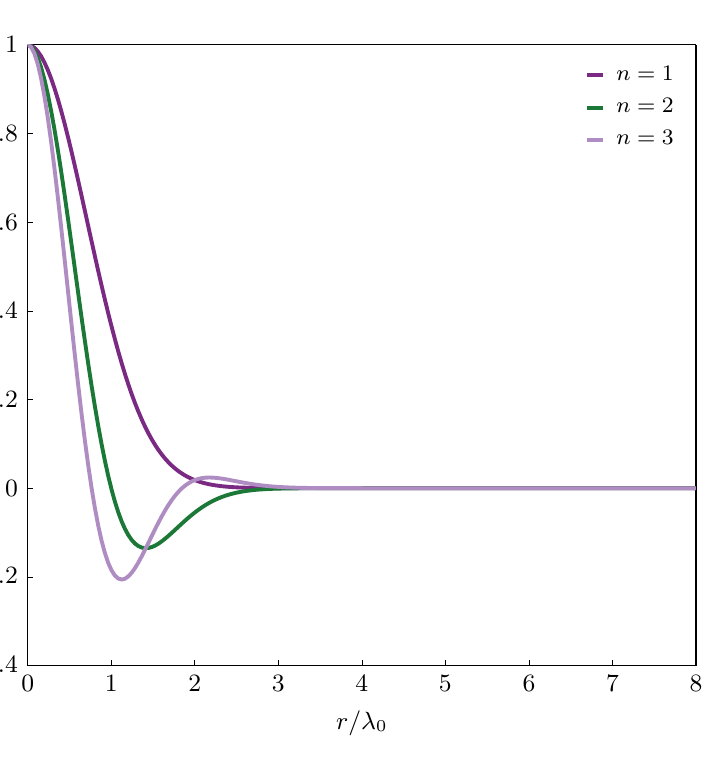
\begin{tikzpicture}[trim axis left,trim axis right]

\begin{axis}[%
width=11.252in,
height=7.131in,
at={(1.887in,0.962in)},
scale only axis,
clip=true,
separate axis lines,
every outer x axis line/.append style={black},
every x tick label/.append style={font=\color{black}},
every x tick/.append style={black},
xmin=0,
xmax=8,
xlabel={$r/\lambda_0$},
every outer y axis line/.append style={black},
every y tick label/.append style={font=\color{black}},
every y tick/.append style={black},
ymin=-0.4,
ymax=1,
ylabel={$C_{00,n}^{xy}(r)$},
axis background/.style={fill=white},
legend style={legend cell align=left, align=left},
clip=true,
clip mode=individual,
axis lines=box,
xtick pos=bottom,
ytick pos=left,
tick align=inside,
major tick length=2pt,
width=0.7\linewidth,
height=0.65\linewidth,
every axis/.append style={font=\fontsize{9}{9}\selectfont},xlabel style={font=\fontsize{9}{9}\selectfont},title style={font=\fontsize{9}{9}\selectfont},
legend style={font=\fontsize{8}{9}\selectfont,inner sep=1pt,row sep=1pt,column sep=2pt,nodes={scale=1.00},draw=none},legend image post style={xscale=0.35},
legend columns=1,
scaled x ticks=false,
tick label style={/pgf/number format/fixed,/pgf/number format/precision=2},
every x tick label/.append style={font=\fontsize{9}{9}\selectfont\color{black}},
every y tick label/.append style={font=\fontsize{9}{9}\selectfont\color{black}},
,,
colormap={sigmamap}{rgb(0.0000)=(0.0200,0.1880,0.3800); rgb(0.1000)=(0.0743,0.3456,0.5616); rgb(0.2000)=(0.1918,0.4980,0.7060); rgb(0.3000)=(0.3890,0.6708,0.8226); rgb(0.4000)=(0.7552,0.8682,0.9228); rgb(0.5000)=(0.9690,0.9689,0.9689); rgb(0.6000)=(0.9425,0.8044,0.7614); rgb(0.7000)=(0.8767,0.4910,0.4020); rgb(0.8000)=(0.7869,0.2866,0.2470); rgb(0.9000)=(0.6186,0.1239,0.1568); rgb(1.0000)=(0.4040,0.0000,0.1220)}
]
\addplot [color=mycolor1, line width=1.4pt]
  table[row sep=crcr]{%
1e-06	0.999999999999\\
0.0400210050025012	0.998399601164802\\
0.0800410100050025	0.993613914988808\\
0.120061015007504	0.985688746313652\\
0.160081020010005	0.974699624420412\\
0.200101025012506	0.960750604625268\\
0.240121030015008	0.943972627966267\\
0.280141035017509	0.924521475140297\\
0.32016104002001	0.902575359394744\\
0.360181045022511	0.878332210368438\\
0.400201050025012	0.852006706724764\\
0.440221055027514	0.823827119687516\\
0.484243060530265	0.79097308236634\\
0.524263065532766	0.759684729113178\\
0.564283070535268	0.727300616844434\\
0.604303075537769	0.6940701748391\\
0.64432308054027	0.660239763357353\\
0.684343085542771	0.626049737144811\\
0.724363090545273	0.59173174103289\\
0.764383095547774	0.557506276865767\\
0.804403100550275	0.523580573109958\\
0.844423105552776	0.490146780255911\\
0.884443110555278	0.457380506752258\\
0.924463115557779	0.425439701962636\\
0.96448312056028	0.39446388472475\\
1.00450312556278	0.364573708720333\\
1.04452313056528	0.335870849201984\\
1.08454313556778	0.308438189804935\\
1.12456314057028	0.282340283299189\\
1.16458314557279	0.257624056274803\\
1.20460315057529	0.234319724928809\\
1.24462315557779	0.212441887331191\\
1.28464316058029	0.191990756752799\\
1.32466316558279	0.172953500776418\\
1.36868517108554	0.153616030642925\\
1.40870517608804	0.137456156692945\\
1.44872518109055	0.122602894026061\\
1.48874518609305	0.109004923383705\\
1.52876519109555	0.096605170968143\\
1.56878519609805	0.0853421343566971\\
1.60880520110055	0.0751511263337177\\
1.64882520610305	0.0659654235207782\\
1.68884521110555	0.0577173101953688\\
1.72886521610805	0.0503390110203401\\
1.76888522111056	0.0437635094916467\\
1.80890522611306	0.0379252516972433\\
1.84892523111556	0.0327607374274328\\
1.88894523611806	0.0282090027635224\\
1.92896524112056	0.0242119999879278\\
1.96898524612306	0.0207148820077474\\
2.00900525112556	0.0176661994786927\\
2.04902525612806	0.0150180194791661\\
2.08904526113057	0.012725974944051\\
2.12906526613307	0.0107492541581323\\
2.16908527113557	0.00905053946678608\\
2.20910527613807	0.00759590402492638\\
2.25312728164082	0.00624120162348047\\
2.29314728664332	0.00520297616216849\\
2.33316729164582	0.00432358823816512\\
2.37318729664832	0.00358134108139998\\
2.41320730165083	0.00295703121831066\\
2.45322730665333	0.0024337446047919\\
2.49324731165583	0.00199665468359556\\
2.53326731665833	0.00163282555159215\\
2.57328732166083	0.00133102275996024\\
2.61330732666333	0.00108153366651469\\
2.65332733166583	0.000875998719344083\\
2.69334733666833	0.000707254577226614\\
2.73336734167084	0.000569189565086317\\
2.77338734667334	0.000456611620243819\\
2.81340735167584	0.000365128604090978\\
2.85342735667834	0.000291040629623266\\
2.89344736168084	0.000231243882767755\\
2.93346736668334	0.000183145288956025\\
2.97348737168584	0.000144587290025496\\
3.01350737668834	0.000113781944435656\\
3.05352738169085	8.92535403114787e-05\\
3.09354738669335	6.97889106716043e-05\\
3.1375693921961	5.3046498924736e-05\\
3.1775893971986	4.1199914486186e-05\\
3.2176094022011	3.18966278072457e-05\\
3.2576294072036	2.46151277540626e-05\\
3.2976494122061	1.89351297201011e-05\\
3.3376694172086	1.45192218940205e-05\\
3.37768942221111	1.1097554015231e-05\\
3.41770942721361	8.45512553019439e-06\\
3.45772943221611	6.42128164882296e-06\\
3.49774943721861	4.8610741519019e-06\\
3.53776944222111	3.66818845661831e-06\\
3.57778944722361	2.75917915890061e-06\\
3.61780945222611	2.06879295846269e-06\\
3.65782945722861	1.54619058659399e-06\\
3.69784946223112	1.15190824727759e-06\\
3.73786946723362	8.55424368192136e-07\\
3.77788947223612	6.33219404399189e-07\\
3.81790947723862	4.6723533522549e-07\\
3.85792948224112	3.43657646102901e-07\\
3.89794948724362	2.51956292962435e-07\\
3.93796949224612	1.84133698326139e-07\\
3.97798949724862	1.34137500465833e-07\\
4.02201150275138	9.43196276680939e-08\\
4.06203150775388	6.82492105497248e-08\\
4.10205151275638	4.92268508511979e-08\\
4.14207151775888	3.53928342989794e-08\\
4.18209152276138	2.53651537421737e-08\\
4.22211152776388	1.8120430961328e-08\\
4.26213153276638	1.29035263483008e-08\\
4.30215153776888	9.1591921633164e-09\\
4.34217154277139	6.48059372303923e-09\\
4.38219154777389	4.57068496023989e-09\\
4.42221155277639	3.21333975834547e-09\\
4.46223155777889	2.25185734354156e-09\\
4.50225156278139	1.57301899928504e-09\\
4.54227156778389	1.09530716668187e-09\\
4.58229157278639	7.60233070441163e-10\\
4.62231157778889	5.2597663614046e-10\\
4.6623315827914	3.6273963865497e-10\\
4.7023515877939	2.49363247995418e-10\\
4.7423715927964	1.70875084877425e-10\\
4.7823915977989	1.16716943962175e-10\\
4.8224116028014	7.9469035013004e-11\\
4.8624316078039	5.39350192834225e-11\\
4.90645361330665	3.50836095281114e-11\\
4.94647361830916	2.36513420422409e-11\\
4.98649362331166	1.58933766667526e-11\\
5.02651362831416	1.06459747216356e-11\\
5.06653363331666	7.1082640536508e-12\\
5.10655363831916	4.73097378204817e-12\\
5.14657364332166	3.13867535609458e-12\\
5.18659364832416	2.07563564786554e-12\\
5.22661365332666	1.36824765173743e-12\\
5.26663365832917	8.99056880984078e-13\\
5.30665366333167	5.88868731658669e-13\\
5.34667366833417	3.84466661568461e-13\\
5.38669367333667	2.50211776318582e-13\\
5.42671367833917	1.62317622470872e-13\\
5.46673368334167	1.04962089263502e-13\\
5.50675368834417	6.76562820137053e-14\\
5.54677369334667	4.34703018874741e-14\\
5.58679369834918	2.78410783066888e-14\\
5.62681370335168	1.77741284597066e-14\\
5.66683370835418	1.13109594300301e-14\\
5.70685371335668	7.17495930073217e-15\\
5.74687371835918	4.53678612841743e-15\\
5.79089572386193	2.73000409792804e-15\\
5.83091572886443	1.71463144696031e-15\\
5.87093573386693	1.07346314241637e-15\\
5.91095573886944	6.69903670730517e-16\\
5.95097574387194	4.1672201538937e-16\\
5.99099574887444	2.58398149592029e-16\\
6.03101575387694	1.59713350705079e-16\\
6.07103575887944	9.84015433414923e-17\\
6.11105576388194	6.04326259970597e-17\\
6.15107576888444	3.69955841911029e-17\\
6.19109577388694	2.25754897281505e-17\\
6.23111577888945	1.37319855590568e-17\\
6.27113578389195	8.32603750963023e-18\\
6.31115578889445	5.03213467220562e-18\\
6.35117579389695	3.03162175470186e-18\\
6.39119579889945	1.82056689621065e-18\\
6.43121580390195	1.08980083300828e-18\\
6.47123580890445	6.50274159901648e-19\\
6.51125581390695	3.86771731816392e-19\\
6.55127581890946	2.29309380300723e-19\\
6.59129582391196	1.35518249587828e-19\\
6.63131582891446	7.98330301173825e-20\\
6.67533783441721	4.44405237063416e-20\\
6.71535783941971	2.60041474190959e-20\\
6.75537784442221	1.51675326273018e-20\\
6.79539784942471	8.81852851361355e-21\\
6.83541785442721	5.11076811135279e-21\\
6.87543785942972	2.95246730096635e-21\\
6.91545786443222	1.70017209473838e-21\\
6.95547786943472	9.75909483367566e-22\\
6.99549787443722	5.5838669301376e-22\\
7.03551787943972	3.18470675439909e-22\\
7.07553788444222	1.81055909834295e-22\\
7.11555788944472	1.02604126765943e-22\\
7.15557789444722	5.79596586689341e-23\\
7.19559789944972	3.2635906260576e-23\\
7.23561790445223	1.83178459397958e-23\\
7.27563790945473	1.02485398559846e-23\\
7.31565791445723	5.71555560072707e-24\\
7.35567791945973	3.17734066173813e-24\\
7.39569792446223	1.76067004143708e-24\\
7.43571792946473	9.72525585628352e-25\\
7.47573793446723	5.35467311999438e-25\\
7.51575793946973	2.93882523083718e-25\\
7.55977994497249	1.51339354258516e-25\\
7.59979994997499	8.2503294939145e-26\\
7.63981995497749	4.48331834106133e-26\\
7.67983995997999	2.4284922874267e-26\\
7.71985996498249	1.31124168431141e-26\\
7.75987996998499	7.05728461628706e-27\\
7.79989997498749	3.78618111991713e-27\\
7.83991997999	2.02476211218377e-27\\
7.8799399849925	1.07933309282375e-27\\
7.919959989995	5.73516408144493e-28\\
7.9599799949975	3.0377013151799e-28\\
8	1.60381089054864e-28\\
};
\addlegendentry{$n=1$}

\addplot [color=mycolor2, line width=1.4pt]
  table[row sep=crcr]{%
1e-06	0.999999999998\\
0.0400210050025012	0.996800483651545\\
0.0800410100050025	0.98724826456394\\
0.120061015007504	0.971480390663682\\
0.160081020010005	0.949722037181622\\
0.200101025012506	0.922281746698046\\
0.240121030015008	0.889544951237612\\
0.280141035017509	0.851965954754393\\
0.32016104002001	0.810058594702914\\
0.360181045022511	0.764385834389475\\
0.400201050025012	0.715548562433984\\
0.440221055027514	0.664173891268017\\
0.484243060530265	0.605496743056042\\
0.524263065532766	0.550884042841713\\
0.564283070535268	0.495716911871969\\
0.604303075537769	0.440608096506016\\
0.64432308054027	0.386139751867212\\
0.684343085542771	0.332854706808546\\
0.724363090545273	0.281248979948098\\
0.764383095547774	0.231765663815864\\
0.804403100550275	0.184790250853524\\
0.844423105552776	0.140647431754698\\
0.884443110555278	0.0995993548719855\\
0.924463115557779	0.0618452964606401\\
0.96448312056028	0.0275226565096869\\
1.00450312556278	-0.00329083525115842\\
1.04452313056528	-0.0305738432035671\\
1.08454313556778	-0.0543572382355185\\
1.12456314057028	-0.0747191698508242\\
1.16458314557279	-0.0917795755422772\\
1.20460315057529	-0.105694305512064\\
1.24462315557779	-0.116649035973267\\
1.28464316058029	-0.124853134646875\\
1.32466316558279	-0.130533628414198\\
1.36868517108554	-0.134152740929596\\
1.40870517608804	-0.135318751000766\\
1.44872518109055	-0.134716630099241\\
1.48874518609305	-0.132589471591537\\
1.52876519109555	-0.129172996938708\\
1.56878519609805	-0.124692282335108\\
1.60880520110055	-0.119359090162107\\
1.64882520610305	-0.113369796992132\\
1.68884521110555	-0.106903894997967\\
1.72886521610805	-0.100123031195721\\
1.76888522111056	-0.0931705390878027\\
1.80890522611306	-0.0861714099803679\\
1.84892523111556	-0.0792326464422981\\
1.88894523611806	-0.0724439378864841\\
1.92896524112056	-0.0658785978650915\\
1.96898524612306	-0.0595947041098592\\
2.00900525112556	-0.0536363853194966\\
2.04902525612806	-0.0480352028889651\\
2.08904526113057	-0.0428115808804694\\
2.12906526613307	-0.0379762432562971\\
2.16908527113557	-0.0335316234539607\\
2.20910527613807	-0.0294732175382701\\
2.25312728164082	-0.0254427736122996\\
2.29314728664332	-0.0221570013462918\\
2.33316729164582	-0.0192125976635722\\
2.37318729664832	-0.0165888361561136\\
2.41320730165083	-0.0142634455382412\\
2.45322730665333	-0.0122133194909206\\
2.49324731165583	-0.0104151141998878\\
2.53326731665833	-0.00884573984070343\\
2.57328732166083	-0.00748275392071925\\
2.61330732666333	-0.00630466551580028\\
2.65332733166583	-0.00529116009842465\\
2.69334733666833	-0.00442325490878138\\
2.73336734167084	-0.00368339473892676\\
2.77338734667334	-0.00305549764820509\\
2.81340735167584	-0.00252495956900456\\
2.85342735667834	-0.00207862605354012\\
2.89344736168084	-0.00170473860658529\\
2.93346736668334	-0.0013928621908675\\
2.97348737168584	-0.00113379961894743\\
3.01350737668834	-0.000919497688415777\\
3.05352738169085	-0.00074294909992025\\
3.09354738669335	-0.000598093437336176\\
3.1375693921961	-0.000469161361993449\\
3.1775893971986	-0.000374798686414659\\
3.2176094022011	-0.000298329487304294\\
3.2576294072036	-0.000236604284356521\\
3.2976494122061	-0.000186974780233718\\
3.3376694172086	-0.000147225449228501\\
3.37768942221111	-0.000115512063013765\\
3.41770942721361	-9.03069782526349e-05\\
3.45772943221611	-7.03508735527202e-05\\
3.49774943721861	-5.46105277624496e-05\\
3.53776944222111	-4.22421709444225e-05\\
3.57778944722361	-3.25599070282465e-05\\
3.61780945222611	-2.50086972552949e-05\\
3.65782945722861	-1.91414008667813e-05\\
3.69784946223112	-1.45993895410912e-05\\
3.73786946723362	-1.10962810350996e-05\\
3.77788947223612	-8.40437216485464e-06\\
3.81790947723862	-6.34338911944219e-06\\
3.85792948224112	-4.77121213076601e-06\\
3.89794948724362	-3.57627019354867e-06\\
3.93796949224612	-2.67133872715635e-06\\
3.97798949724862	-1.98850802095575e-06\\
4.02201150275138	-1.43144904742223e-06\\
4.06203150775388	-1.05786958639331e-06\\
4.10205151275638	-7.79104833141027e-07\\
4.14207151775888	-5.71833404135077e-07\\
4.18209152276138	-4.18268582479506e-07\\
4.22211152776388	-3.04898462094721e-07\\
4.26213153276638	-2.21498903580513e-07\\
4.30215153776888	-1.60363787927053e-07\\
4.34217154277139	-1.1570746062093e-07\\
4.38219154777389	-8.3202933363625e-08\\
4.42221155277639	-5.96265880118317e-08\\
4.46223155777889	-4.25860237411274e-08\\
4.50225156278139	-3.03124994700107e-08\\
4.54227156778389	-2.15033233073229e-08\\
4.58229157278639	-1.52026818060235e-08\\
4.62231157778889	-1.07119162105998e-08\\
4.6623315827914	-7.52225369036748e-09\\
4.7023515877939	-5.26458443515363e-09\\
4.7423715927964	-3.67212066641458e-09\\
4.7823915977989	-2.55274772432255e-09\\
4.8224116028014	-1.76863532048689e-09\\
4.8624316078039	-1.22126364755585e-09\\
4.90645361330665	-8.09494193726573e-10\\
4.94647361830916	-5.55040264231443e-10\\
4.98649362331166	-3.7929731998587e-10\\
5.02651362831416	-2.58333511314688e-10\\
5.06653363331666	-1.75359189953915e-10\\
5.10655363831916	-1.1863810941404e-10\\
5.14657364332166	-7.99961101446666e-11\\
5.18659364832416	-5.37605276299237e-11\\
5.22661365332666	-3.60088442767934e-11\\
5.26663365832917	-2.40384705031853e-11\\
5.30665366333167	-1.5994012234022e-11\\
5.34667366833417	-1.06062507722495e-11\\
5.38669367333667	-7.0100504071987e-12\\
5.42671367833917	-4.61780997013962e-12\\
5.46673368334167	-3.03184854394097e-12\\
5.50675368834417	-1.98397555873564e-12\\
5.54677369334667	-1.29396736586755e-12\\
5.58679369834918	-8.41142003055296e-13\\
5.62681370335168	-5.44973129513101e-13\\
5.66683370835418	-3.51917929136384e-13\\
5.70685371335668	-2.26500401716275e-13\\
5.74687371835918	-1.45297641964696e-13\\
5.79089572386193	-8.8819245391004e-14\\
5.83091572886443	-5.65821145817908e-14\\
5.87093573386693	-3.59265424955271e-14\\
5.91095573886944	-2.27361271330136e-14\\
5.95097574387194	-1.43411182372224e-14\\
5.99099574887444	-9.0160360037968e-15\\
6.03101575387694	-5.64956447496186e-15\\
6.07103575887944	-3.5284308985916e-15\\
6.11105576388194	-2.1964239459225e-15\\
6.15107576888444	-1.3627594656806e-15\\
6.19109577388694	-8.42735511237248e-16\\
6.23111577888945	-5.19437124212444e-16\\
6.27113578389195	-3.19113238747604e-16\\
6.31115578889445	-1.95401248369331e-16\\
6.35117579389695	-1.19256220582389e-16\\
6.39119579889945	-7.25448277374096e-17\\
6.43121580390195	-4.39849465341486e-17\\
6.47123580890445	-2.65811871863263e-17\\
6.51125581390695	-1.60109775371226e-17\\
6.55127581890946	-9.61246918119099e-18\\
6.59129582391196	-5.7520965835442e-18\\
6.63131582891446	-3.43077254771283e-18\\
6.67533783441721	-1.93583522116711e-18\\
6.71535783941971	-1.1466796884185e-18\\
6.75537784442221	-6.7700478788251e-19\\
6.79539784942471	-3.98398471663878e-19\\
6.83541785442721	-2.33679329627201e-19\\
6.87543785942972	-1.3661552106499e-19\\
6.91545786443222	-7.9608105794927e-20\\
6.95547786943472	-4.62372956969093e-20\\
6.99549787443722	-2.6767377604612e-20\\
7.03551787943972	-1.54453538209407e-20\\
7.07553788444222	-8.8831888975206e-21\\
7.11555788944472	-5.09236225060441e-21\\
7.15557789444722	-2.9097078828001e-21\\
7.19559789944972	-1.65714130853316e-21\\
7.23561790445223	-9.40697709566797e-22\\
7.27563790945473	-5.3225696419869e-22\\
7.31565791445723	-3.00174411384222e-22\\
7.35567791945973	-1.68735845730853e-22\\
7.39569792446223	-9.45415508882542e-23\\
7.43571792946473	-5.27983178868163e-23\\
7.47573793446723	-2.93900110444211e-23\\
7.51575793946973	-1.63065471202749e-23\\
7.55977994497249	-8.49774602947474e-24\\
7.59979994997499	-4.68263615129716e-24\\
7.63981995497749	-2.57193846041647e-24\\
7.67983995997999	-1.40803841513233e-24\\
7.71985996498249	-7.68338296506925e-25\\
7.75987996998499	-4.17902310820732e-25\\
7.79989997498749	-2.26559170333825e-25\\
7.83991997999	-1.22425915486547e-25\\
7.8799399849925	-6.59401868374441e-26\\
7.919959989995	-3.54007397457217e-26\\
7.9599799949975	-1.89434946891918e-26\\
8	-1.01040086104564e-26\\
};
\addlegendentry{$n=2$}

\addplot [color=mycolor3, line width=1.4pt]
  table[row sep=crcr]{%
1e-06	0.999999999997\\
0.0400210050025012	0.99520264677623\\
0.0800410100050025	0.980903005110212\\
0.120061015007504	0.957374439231591\\
0.160081020010005	0.925064486930967\\
0.200101025012506	0.884583043389047\\
0.240121030015008	0.836686372969184\\
0.280141035017509	0.782257476692557\\
0.32016104002001	0.722283457211489\\
0.360181045022511	0.65783061203409\\
0.400201050025012	0.590018046409692\\
0.440221055027514	0.519990627805751\\
0.484243060530265	0.44176670157236\\
0.524263065532766	0.37077797482217\\
0.564283070535268	0.301003114037397\\
0.604303075537769	0.233425938764405\\
0.64432308054027	0.168936356173771\\
0.684343085542771	0.108315025012104\\
0.724363090545273	0.0522216641657382\\
0.764383095547774	0.0011871604973946\\
0.804403100550275	-0.0443905018834978\\
0.844423105552776	-0.0842465949090469\\
0.884443110555278	-0.118246501613079\\
0.924463115557779	-0.146379392601539\\
0.96448312056028	-0.168749126189556\\
1.00450312556278	-0.185562837200974\\
1.04452313056528	-0.197117721187076\\
1.08454313556778	-0.203786541461311\\
1.12456314057028	-0.206002386620344\\
1.16458314557279	-0.204243187680562\\
1.20460315057529	-0.199016468821881\\
1.24462315557779	-0.19084475673101\\
1.28464316058029	-0.180252013757371\\
1.32466316558279	-0.167751392801878\\
1.36868517108554	-0.152383022457257\\
1.40870517608804	-0.137439538655591\\
1.44872518109055	-0.122004447297636\\
1.48874518609305	-0.106453520672244\\
1.52876519109555	-0.0911154892160205\\
1.56878519609805	-0.0762702136835455\\
1.60880520110055	-0.0621483666866192\\
1.64882520610305	-0.0489324500001596\\
1.68884521110555	-0.0367589519805289\\
1.72886521610805	-0.0257214369501888\\
1.76888522111056	-0.0158743547841\\
1.80890522611306	-0.00723736322042795\\
1.84892523111556	0.00020003356054727\\
1.88894523611806	0.00647371008769024\\
1.92896524112056	0.0116401679354758\\
1.96898524612306	0.0157719434090352\\
2.00900525112556	0.0189532859681485\\
2.04902525612806	0.0212761936768565\\
2.08904526113057	0.0228368675313141\\
2.12906526613307	0.023732623581764\\
2.16908527113557	0.0240592809691401\\
2.20910527613807	0.0239090258024204\\
2.25312728164082	0.0232964090070341\\
2.29314728664332	0.02241957687141\\
2.33316729164582	0.0213128264084734\\
2.37318729664832	0.0200403866838539\\
2.41320730165083	0.0186583991468383\\
2.45322730665333	0.0172150066990815\\
2.49324731165583	0.0157506456407219\\
2.53326731665833	0.0142984943898845\\
2.57328732166083	0.0128850362784983\\
2.61330732666333	0.0115306980002704\\
2.65332733166583	0.010250530105904\\
2.69334733666833	0.0090549010232812\\
2.73336734167084	0.0079501811855913\\
2.77338734667334	0.00693939878212585\\
2.81340735167584	0.00602285325316882\\
2.85342735667834	0.00519867682311919\\
2.89344736168084	0.00446333803466766\\
2.93346736668334	0.00381208437573296\\
2.97348737168584	0.00323932367309791\\
3.01350737668834	0.0027389459787743\\
3.05352738169085	0.00230458923142039\\
3.09354738669335	0.0019298530826504\\
3.1375693921961	0.00157902708535051\\
3.1775893971986	0.00130938711973568\\
3.2176094022011	0.00108086157736653\\
3.2576294072036	0.000888226011362204\\
3.2976494122061	0.000726698107604974\\
3.3376694172086	0.000591950701284288\\
3.37768942221111	0.000480109322492955\\
3.41770942721361	0.000387738033883611\\
3.45772943221611	0.000311816801066955\\
3.49774943721861	0.000249713126653047\\
3.53776944222111	0.000199150197589604\\
3.57778944722361	0.00015817335374278\\
3.61780945222611	0.000125116290255197\\
3.65782945722861	9.85680603628926e-05\\
3.69784946223112	7.73416495403549e-05\\
3.73786946723362	6.04446444466514e-05\\
3.77788947223612	4.70523180307922e-05\\
3.81790947723862	3.64832911902355e-05\\
3.85792948224112	2.8177806865108e-05\\
3.89794948724362	2.16785594716875e-05\\
3.93796949224612	1.66139562539033e-05\\
3.97798949724862	1.26836428194304e-05\\
4.02201150275138	9.38363914600103e-06\\
4.06203150775388	7.10654798048342e-06\\
4.10205151275638	5.36166029528959e-06\\
4.14207151775888	4.02995670136077e-06\\
4.18209152276138	3.01765019484769e-06\\
4.22211152776388	2.25118649987996e-06\\
4.26213153276638	1.67314841899372e-06\\
4.30215153776888	1.23892193619445e-06\\
4.34217154277139	9.13998992114544e-07\\
4.38219154777389	6.71808297922792e-07\\
4.42221155277639	4.91980884606539e-07\\
4.46223155777889	3.5897106462663e-07\\
4.50225156278139	2.60966002494617e-07\\
4.54227156778389	1.89028128279455e-07\\
4.58229157278639	1.3642422626838e-07\\
4.62231157778889	9.8103275963237e-08\\
4.6623315827914	7.02921268197431e-08\\
4.7023515877939	5.01839779887669e-08\\
4.7423715927964	3.56995405202621e-08\\
4.7823915977989	2.53048103913761e-08\\
4.8224116028014	1.78726977398493e-08\\
4.8624316078039	1.25784524767123e-08\\
4.90645361330665	8.51180995394734e-09\\
4.94647361830916	5.94586586592604e-09\\
4.98649362331166	4.13874376523606e-09\\
5.02651362831416	2.87068323127658e-09\\
5.06653363331666	1.9841215110809e-09\\
5.10655363831916	1.36653381710714e-09\\
5.14657364332166	9.37873792022771e-10\\
5.18659364832416	6.41420746278332e-10\\
5.22661365332666	4.37138236542148e-10\\
5.26663365832917	2.96875463343613e-10\\
5.30665366333167	2.00914822642777e-10\\
5.34667366833417	1.35498408044807e-10\\
5.38669367333667	9.10632727204254e-11\\
5.42671367833917	6.09875802073137e-11\\
5.46673368334167	4.07034115753854e-11\\
5.50675368834417	2.70715794329505e-11\\
5.54677369334667	1.79428656461657e-11\\
5.58679369834918	1.18513395143147e-11\\
5.62681370335168	7.80085921105328e-12\\
5.66683370835418	5.1170386085357e-12\\
5.70685371335668	3.34501476572425e-12\\
5.74687371835918	2.17912560999528e-12\\
5.79089572386193	1.35465943572789e-12\\
5.83091572886443	8.76153528176437e-13\\
5.87093573386693	5.64729447267646e-13\\
5.91095573886944	3.62754152027037e-13\\
5.95097574387194	2.32218947546531e-13\\
5.99099574887444	1.48148664568334e-13\\
6.03101575387694	9.41920275446321e-14\\
6.07103575887944	5.96826800249013e-14\\
6.11105576388194	3.76878766979996e-14\\
6.15107576888444	2.37178647307976e-14\\
6.19109577388694	1.48754946957223e-14\\
6.23111577888945	9.29801998798465e-15\\
6.27113578389195	5.79207327258321e-15\\
6.31115578889445	3.59586507998287e-15\\
6.35117579389695	2.22484481957682e-15\\
6.39119579889945	1.37190568341215e-15\\
6.43121580390195	8.43098177828627e-16\\
6.47123580890445	5.1637184654508e-16\\
6.51125581390695	3.15194470335858e-16\\
6.55127581890946	1.9174645657742e-16\\
6.59129582391196	1.16254533560458e-16\\
6.63131582891446	7.02469204081058e-17\\
6.67533783441721	4.02045664999467e-17\\
6.71535783941971	2.41223297308923e-17\\
6.75537784442221	1.44245097440607e-17\\
6.79539784942471	8.59650218177638e-18\\
6.83541785442721	5.10601794827208e-18\\
6.87543785942972	3.02262074322651e-18\\
6.91545786443222	1.78330916672957e-18\\
6.95547786943472	1.04860559212389e-18\\
6.99549787443722	6.14527192170623e-19\\
7.03551787943972	3.58933748357849e-19\\
7.07553788444222	2.0894528137649e-19\\
7.11555788944472	1.21226268888292e-19\\
7.15557789444722	7.0098319041038e-20\\
7.19559789944972	4.03985655585005e-20\\
7.23561790445223	2.3204516749918e-20\\
7.27563790945473	1.32839767309582e-20\\
7.31565791445723	7.57937536174555e-21\\
7.35567791945973	4.31011819777227e-21\\
7.39569792446223	2.4428461126369e-21\\
7.43571792946473	1.37992314818243e-21\\
7.47573793446723	7.76901992779973e-22\\
7.51575793946973	4.35944082245404e-22\\
7.55977994497249	2.30001963233174e-22\\
7.59979994997499	1.28162206881505e-22\\
7.63981995497749	7.11776475244733e-23\\
7.67983995997999	3.93988118118765e-23\\
7.71985996498249	2.1735972291881e-23\\
7.75987996998499	1.19517657425422e-23\\
7.79989997498749	6.55002135627364e-24\\
7.83991997999	3.57776311683082e-24\\
7.8799399849925	1.9477770377773e-24\\
7.919959989995	1.05688139523921e-24\\
7.9599799949975	5.71574922894909e-25\\
8	3.08092072074393e-25\\
};
\addlegendentry{$n=3$}

\node[overlay,right, align=left, inner sep=0]
at (rel axis cs:-0.15,1.1) {$(a)$};
\end{axis}
\end{tikzpicture}%
  \end{minipage}
  \hfill
  \begin{minipage}{0.48\textwidth}
    \centering
    % This file was created by matlab2tikz.
%
\definecolor{mycolor1}{rgb}{0.48200,0.16500,0.51400}%
\definecolor{mycolor2}{rgb}{0.10600,0.47100,0.21600}%
\definecolor{mycolor3}{rgb}{0.68600,0.55300,0.76500}%
%
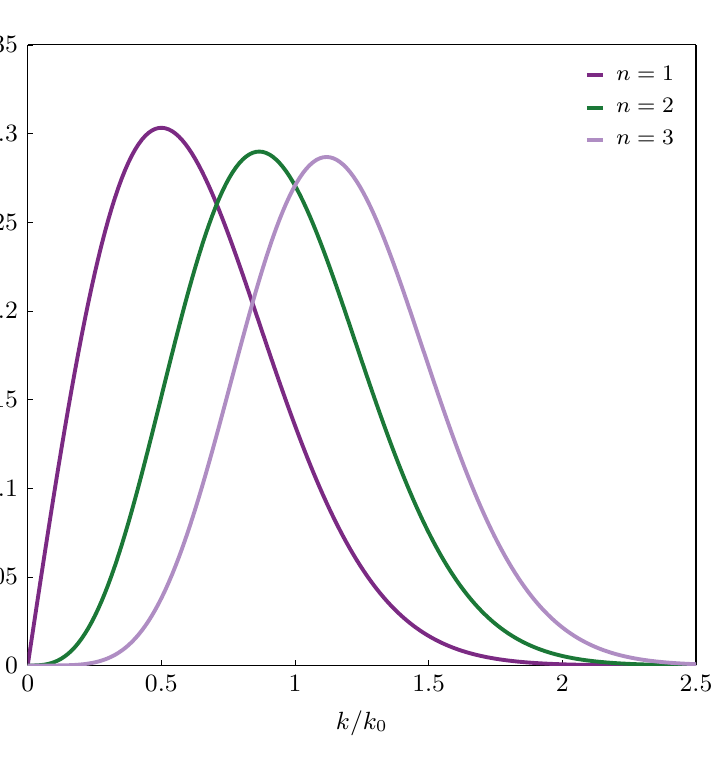
\begin{tikzpicture}[trim axis left,trim axis right]

\begin{axis}[%
width=11.252in,
height=7.131in,
at={(1.887in,0.962in)},
scale only axis,
clip=true,
separate axis lines,
every outer x axis line/.append style={black},
every x tick label/.append style={font=\color{black}},
every x tick/.append style={black},
xmin=0,
xmax=2.5,
xlabel={$k/k_0$},
every outer y axis line/.append style={black},
every y tick label/.append style={font=\color{black}},
every y tick/.append style={black},
ymin=0,
ymax=0.35,
ylabel={$E_{\eta,n}(k)$},
axis background/.style={fill=white},
legend style={legend cell align=left, align=left},
clip=true,
clip mode=individual,
axis lines=box,
xtick pos=bottom,
ytick pos=left,
tick align=inside,
major tick length=2pt,
width=0.7\linewidth,
height=0.65\linewidth,
every axis/.append style={font=\fontsize{9}{9}\selectfont},xlabel style={font=\fontsize{9}{9}\selectfont},title style={font=\fontsize{9}{9}\selectfont},
legend style={font=\fontsize{8}{9}\selectfont,inner sep=1pt,row sep=1pt,column sep=2pt,nodes={scale=1.00},draw=none},legend image post style={xscale=0.35},
legend columns=1,
scaled x ticks=false,
tick label style={/pgf/number format/fixed,/pgf/number format/precision=2},
every x tick label/.append style={font=\fontsize{9}{9}\selectfont\color{black}},
every y tick label/.append style={font=\fontsize{9}{9}\selectfont\color{black}},
,,
colormap={sigmamap}{rgb(0.0000)=(0.0200,0.1880,0.3800); rgb(0.1000)=(0.0743,0.3456,0.5616); rgb(0.2000)=(0.1918,0.4980,0.7060); rgb(0.3000)=(0.3890,0.6708,0.8226); rgb(0.4000)=(0.7552,0.8682,0.9228); rgb(0.5000)=(0.9690,0.9689,0.9689); rgb(0.6000)=(0.9425,0.8044,0.7614); rgb(0.7000)=(0.8767,0.4910,0.4020); rgb(0.8000)=(0.7869,0.2866,0.2470); rgb(0.9000)=(0.6186,0.1239,0.1568); rgb(1.0000)=(0.4040,0.0000,0.1220)}
]
\addplot [color=mycolor1, line width=1.4pt]
  table[row sep=crcr]{%
1e-06	9.99999999998e-07\\
0.012507248124062	0.0125033356870642\\
0.0250134962481241	0.0249822151857268\\
0.0375197443721861	0.0374142575081492\\
0.0500259924962481	0.049776227988151\\
0.0625322406203102	0.0620451106388611\\
0.0750384887443722	0.074198179555138\\
0.0875447368684342	0.0862130690507178\\
0.100050984992496	0.0980678422271457\\
0.112557233116558	0.109741057680322\\
0.12506348124062	0.121211834060891\\
0.137569729364682	0.132459912216648\\
0.151326602301151	0.144552237739127\\
0.163832850425213	0.15526980755966\\
0.176339098549275	0.165706455442367\\
0.188845346673337	0.175845062145538\\
0.201351594797399	0.185669401013813\\
0.213857842921461	0.195164180365556\\
0.226364091045523	0.204315081990821\\
0.238870339169585	0.213108795630047\\
0.251376587293647	0.221533049324865\\
0.263882835417709	0.229576635554121\\
0.276389083541771	0.237229433090159\\
0.288895331665833	0.244482424532426\\
0.301401579789895	0.251327709497517\\
0.313907827913957	0.257758513466586\\
0.326414076038019	0.26376919231265\\
0.338920324162081	0.269355232551407\\
0.351426572286143	0.274513247379763\\
0.363932820410205	0.279240968586193\\
0.376439068534267	0.283537234436133\\
0.388945316658329	0.287401973653864\\
0.401451564782391	0.290836185639548\\
0.413957812906453	0.293841917076269\\
0.427714685842921	0.296657016968592\\
0.440220933966983	0.298774103791276\\
0.452727182091046	0.300475402147823\\
0.465233430215107	0.301766937984341\\
0.47773967833917	0.302655615812989\\
0.490245926463232	0.303149177432573\\
0.502752174587294	0.303256158493771\\
0.515258422711356	0.302985843147067\\
0.527764670835418	0.302348217015337\\
0.54027091895948	0.30135391873543\\
0.552777167083542	0.300014190314105\\
0.565283415207604	0.298340826543286\\
0.577789663331666	0.296346123717858\\
0.590295911455728	0.2940428278962\\
0.60280215957979	0.291444082939338\\
0.615308407703852	0.288563378559127\\
0.627814655827914	0.285414498599276\\
0.640320903951976	0.282011469765338\\
0.652827152076038	0.278368511011214\\
0.6653334002001	0.274499983780127\\
0.677839648324162	0.270420343287768\\
0.690345896448224	0.266144091024213\\
0.704102769384692	0.261230433566072\\
0.716609017508754	0.256588445151956\\
0.729115265632816	0.251794604352604\\
0.741621513756878	0.24686313763554\\
0.75412776188094	0.241808100063135\\
0.766634010005002	0.23664333833741\\
0.779140258129065	0.231382455957741\\
0.791646506253126	0.226038780563521\\
0.804152754377189	0.220625333520528\\
0.816659002501251	0.215154801796455\\
0.829165250625313	0.209639512158135\\
0.841671498749375	0.204091407710348\\
0.854177746873437	0.19852202678381\\
0.866683994997499	0.192942484168157\\
0.879190243121561	0.187363454674395\\
0.891696491245623	0.181795159000548\\
0.904202739369685	0.176247351864029\\
0.916708987493747	0.170729312354729\\
0.929215235617809	0.165249836453935\\
0.941721483741871	0.159817231655987\\
0.954227731865933	0.154439313622079\\
0.966733979989995	0.149123404788854\\
0.980490852926463	0.143355662283408\\
0.992997101050525	0.138191618138487\\
1.00550334917459	0.13310916348621\\
1.01800959729865	0.128113622286538\\
1.03051584542271	0.123209845332416\\
1.04302209354677	0.11840221880887\\
1.05552834167084	0.113694674126555\\
1.0680345897949	0.109090698924165\\
1.08054083791896	0.104593349133712\\
1.09304708604302	0.100205262002926\\
1.10555333416708	0.0959286699697512\\
1.11805958229115	0.0917654152852739\\
1.13056583041521	0.0877169652831892\\
1.14307207853927	0.0837844281962175\\
1.15557832666333	0.0799685694225552\\
1.16808457478739	0.0762698281485362\\
1.18059082291146	0.0726883342371032\\
1.19309707103552	0.0692239252954183\\
1.20560331915958	0.0658761638389392\\
1.21810956728364	0.0626443544735069\\
1.2306158154077	0.0595275610214065\\
1.24312206353177	0.0565246235219153\\
1.25687893646823	0.0533512586932931\\
1.2693851845923	0.050582742554742\\
1.28189143271636	0.04792324446996\\
1.29439768084042	0.0453708597065667\\
1.30690392896448	0.0429235422940296\\
1.31941017708854	0.0405791200311605\\
1.33191642521261	0.038335309011414\\
1.34442267333667	0.0361897276348124\\
1.35692892146073	0.0341399100797784\\
1.36943516958479	0.0321833192124766\\
1.38194141770885	0.0303173589154311\\
1.39444766583292	0.028539385821176\\
1.40695391395698	0.0268467204405133\\
1.41946016208104	0.025236657678563\\
1.4319664102051	0.0237064767352062\\
1.44447265832916	0.022253450389725\\
1.45697890645323	0.020874853672428\\
1.46948515457729	0.0195679719288212\\
1.48199140270135	0.0183301082844277\\
1.49449765082541	0.0171585905206906\\
1.50700389894947	0.0160507773744975\\
1.51951014707354	0.015004064275758\\
1.53326702001	0.0139201932227356\\
1.54577326813407	0.0129935043648222\\
1.55827951625813	0.0121201276874942\\
1.57078576438219	0.0112976577428226\\
1.58329201250625	0.0105237469402583\\
1.59579826063032	0.0097961082518346\\
1.60830450875438	0.00911251749448843\\
1.62081075687844	0.00847081521196432\\
1.6333170050025	0.00786890817898354\\
1.64582325312656	0.00730477055043469\\
1.65832950125063	0.00677644467828962\\
1.67083574937469	0.00628204161877771\\
1.68334199749875	0.00581974135207076\\
1.69584824562281	0.00538779273635341\\
1.70835449374687	0.00498451321768748\\
1.72086074187094	0.00460828831653454\\
1.733366989995	0.00425757091118747\\
1.74587323811906	0.00393088033768892\\
1.75837948624312	0.00362680132509161\\
1.77088573436718	0.00334398278414903\\
1.78339198249125	0.00308113646672591\\
1.79589823061531	0.00283703551239094\\
1.80965510355178	0.0025887842603378\\
1.82216135167584	0.00238031932361065\\
1.8346675997999	0.00218716939922618\\
1.84717384792396	0.00200834229180101\\
1.85968009604802	0.00184289856882796\\
1.87218634417209	0.00168994972555733\\
1.88469259229615	0.00154865632932159\\
1.89719884042021	0.00141822615287879\\
1.90970508854427	0.00129791230555245\\
1.92221133666833	0.00118701137017154\\
1.9347175847924	0.00108486155306661\\
1.94722383291646	0.000990840853659224\\
1.95973008104052	0.000904365259492857\\
1.97223632916458	0.000824886971896154\\
1.98474257728864	0.000751892666844868\\
1.99724882541271	0.000684901794997244\\
2.00975507353677	0.00062346492432005\\
2.02226132166083	0.000567162128198694\\
2.03476756978489	0.000515601421434883\\
2.04727381790895	0.000468417246079032\\
2.05978006603302	0.000425269008621212\\
2.07228631415708	0.00038583966967374\\
2.08604318709355	0.000346411460523943\\
2.09854943521761	0.000313856995799808\\
2.11105568334167	0.000284173937835262\\
2.12356193146573	0.000257128211923276\\
2.13606817958979	0.000232502938143593\\
2.14857442771386	0.00021009734700092\\
2.16108067583792	0.000189725746983587\\
2.17358692396198	0.000171216543082732\\
2.18609317208604	0.000154411305167679\\
2.19859942021011	0.00013916388498924\\
2.21110566833417	0.000125339580478016\\
2.22361191645823	0.000112814345917912\\
2.23611816458229	0.000101474046504826\\
2.24862441270635	9.12137557453812e-05\\
2.26113066083042	8.19370941095129e-05\\
2.27363690895448	7.35556073223929e-05\\
2.28614315707854	6.59881826644289e-05\\
2.2986494052026	5.91605016418098e-05\\
2.31115565332666	5.30045273931476e-05\\
2.32366190145073	4.74580252092345e-05\\
2.33616814957479	4.2464114561786e-05\\
2.34867439769885	3.79708510623788e-05\\
2.36243127063532	3.35500659514266e-05\\
2.37493751875938	2.99588643141167e-05\\
2.38744376688344	2.67345922799202e-05\\
2.3999500150075	2.38417517501924e-05\\
2.41245626313157	2.12480587809647e-05\\
2.42496251125563	1.89241760545548e-05\\
2.43746875937969	1.68434651930235e-05\\
2.44997500750375	1.49817576851635e-05\\
2.46248125562781	1.33171432506067e-05\\
2.47498750375188	1.182977451687e-05\\
2.48749375187594	1.05016869373549e-05\\
2.5	9.31663293019668e-06\\
};
\addlegendentry{$n=1$}

\addplot [color=mycolor2, line width=1.4pt]
  table[row sep=crcr]{%
1e-06	1.999999999996e-18\\
0.012507248124062	3.91182500235304e-06\\
0.0250134962481241	3.12614947005987e-05\\
0.0375197443721861	0.000105338436566632\\
0.0500259924962481	0.000249139968883221\\
0.0625322406203102	0.000485227649066178\\
0.0750384887443722	0.000835586478256945\\
0.0875447368684342	0.00132148788088522\\
0.100050984992496	0.00196335734967166\\
0.112557233116558	0.00278064761171072\\
0.12506348124062	0.00379171813014021\\
0.137569729364682	0.00501372170881961\\
0.151326602301151	0.00662041748434639\\
0.163832850425213	0.00833525681121348\\
0.176339098549275	0.0103054427723424\\
0.188845346673337	0.0125421719033817\\
0.201351594797399	0.0150549902831408\\
0.213857842921461	0.0178517366579682\\
0.226364091045523	0.02093849634428\\
0.238870339169585	0.0243195661344885\\
0.251376587293647	0.0279974303533997\\
0.263882835417709	0.0319727481335621\\
0.276389083541771	0.036244351899698\\
0.288895331665833	0.0408092569748465\\
0.301401579789895	0.0456626821448074\\
0.313907827913957	0.0507980809434863\\
0.326414076038019	0.056207183350368\\
0.338920324162081	0.0618800475231208\\
0.351426572286143	0.0678051211237688\\
0.363932820410205	0.0739693117364142\\
0.376439068534267	0.0803580658185823\\
0.388945316658329	0.0869554555772692\\
0.401451564782391	0.0937442731150242\\
0.413957812906453	0.100706131151188\\
0.427714685842921	0.108540781846169\\
0.440220933966983	0.115801538607845\\
0.452727182091046	0.123172019498758\\
0.465233430215107	0.130630166447205\\
0.47773967833917	0.138153330169548\\
0.490245926463232	0.145718394385814\\
0.502752174587294	0.153301901038872\\
0.515258422711356	0.160880175717106\\
0.527764670835418	0.168429452494566\\
0.54027091895948	0.175925997422113\\
0.552777167083542	0.183346229927788\\
0.565283415207604	0.190666841414204\\
0.577789663331666	0.197864910374866\\
0.590295911455728	0.204918013389573\\
0.60280215957979	0.211804331401061\\
0.615308407703852	0.218502750720376\\
0.627814655827914	0.224992958256707\\
0.640320903951976	0.231255530518063\\
0.652827152076038	0.237272015981847\\
0.6653334002001	0.243025010488528\\
0.677839648324162	0.248498225366866\\
0.690345896448224	0.253676548054941\\
0.704102769384692	0.259015570360991\\
0.716609017508754	0.263530950488702\\
0.729115265632816	0.267712591193295\\
0.741621513756878	0.271550670738605\\
0.75412776188094	0.275036731399896\\
0.766634010005002	0.278163692429428\\
0.779140258129065	0.280925855405849\\
0.791646506253126	0.283318902153342\\
0.804152754377189	0.285339885459202\\
0.816659002501251	0.286987212858155\\
0.829165250625313	0.288260623788246\\
0.841671498749375	0.289161160456131\\
0.854177746873437	0.289691132779161\\
0.866683994997499	0.289854077797518\\
0.879190243121561	0.28965471397187\\
0.891696491245623	0.289098890800455\\
0.904202739369685	0.288193534204232\\
0.916708987493747	0.286946588139744\\
0.929215235617809	0.285366952906717\\
0.941721483741871	0.283464420621233\\
0.954227731865933	0.281249608325641\\
0.966733979989995	0.278733889203472\\
0.980490852926463	0.275633462054939\\
0.992997101050525	0.272525822525016\\
1.00550334917459	0.269156574707533\\
1.01800959729865	0.265539449734544\\
1.03051584542271	0.261688571204898\\
1.04302209354677	0.25761838441254\\
1.05552834167084	0.253343586669873\\
1.0680345897949	0.248879059071574\\
1.08054083791896	0.244239800020315\\
1.09304708604302	0.239440860810677\\
1.10555333416708	0.234497283541543\\
1.11805958229115	0.229424041600589\\
1.13056583041521	0.224235982937377\\
1.14307207853927	0.218947776314266\\
1.15557832666333	0.213573860697076\\
1.16808457478739	0.208128397920342\\
1.18059082291146	0.202625228735368\\
1.19309707103552	0.197077832323188\\
1.20560331915958	0.191499289329223\\
1.21810956728364	0.18590224845199\\
1.2306158154077	0.18029889659484\\
1.24312206353177	0.17470093256743\\
1.25687893646823	0.168562732150052\\
1.2693851845923	0.163011866002044\\
1.28189143271636	0.157499325565096\\
1.29439768084042	0.152034607235555\\
1.30690392896448	0.146626638441337\\
1.31941017708854	0.141283771586688\\
1.33191642521261	0.136013780932139\\
1.34442267333667	0.130823862268147\\
1.35692892146073	0.125720635232066\\
1.36943516958479	0.120710148110709\\
1.38194141770885	0.115797884964886\\
1.39444766583292	0.110988774907839\\
1.40695391395698	0.106287203366435\\
1.41946016208104	0.101697025152242\\
1.4319664102051	0.0972215791690861\\
1.44447265832916	0.092863704584415\\
1.45697890645323	0.0886257582935311\\
1.46948515457729	0.084509633508598\\
1.48199140270135	0.0805167793080312\\
1.49449765082541	0.0766482209864793\\
1.50700389894947	0.0729045810509312\\
1.51951014707354	0.0692861007145002\\
1.53326702001	0.0654501803871208\\
1.54577326813407	0.0620937483722139\\
1.55827951625813	0.0588610377416395\\
1.57078576438219	0.0557509565170094\\
1.58329201250625	0.052762143839635\\
1.59579826063032	0.0498929917026545\\
1.60830450875438	0.0471416663392376\\
1.62081075687844	0.0445061291813547\\
1.6333170050025	0.0419841573119727\\
1.64582325312656	0.0395733633418135\\
1.65832950125063	0.0372712146499506\\
1.67083574937469	0.0350750519354708\\
1.68334199749875	0.0329821070351399\\
1.69584824562281	0.0309895199694631\\
1.70835449374687	0.0290943551866689\\
1.72086074187094	0.0272936169809641\\
1.733366989995	0.0255842640678607\\
1.74587323811906	0.0239632233054625\\
1.75837948624312	0.0224274025562953\\
1.77088573436718	0.020973702689564\\
1.78339198249125	0.0195990287286103\\
1.79589823061531	0.0183003001528321\\
1.80965510355178	0.0169557685220001\\
1.82216135167584	0.0158066151622171\\
1.8346675997999	0.0147240471498316\\
1.84717384792396	0.0137051335517257\\
1.85968009604802	0.0127469978986512\\
1.87218634417209	0.0118468237386303\\
1.88469259229615	0.0110018595047996\\
1.89719884042021	0.0102094227289079\\
1.90970508854427	0.00946690363279301\\
1.92221133666833	0.0087717681309781\\
1.9347175847924	0.00812156027807352\\
1.94722383291646	0.0075139041949537\\
1.95973008104052	0.00694650550772695\\
1.97223632916458	0.00641715233334719\\
1.98474257728864	0.00592371584535152\\
1.99724882541271	0.00546415045266323\\
2.00975507353677	0.00503649362369966\\
2.02226132166083	0.00463886538718285\\
2.03476756978489	0.0042694675400896\\
2.04727381790895	0.003926582592112\\
2.05978006603302	0.00360857247484645\\
2.07228631415708	0.00331387704270614\\
2.08604318709355	0.00301487171909493\\
2.09854943521761	0.00276439575655084\\
2.11105568334167	0.00253287419120097\\
2.12356193146573	0.00231904719951338\\
2.13606817958979	0.00212172289180142\\
2.14857442771386	0.00193977504995146\\
2.16108067583792	0.00177214081014392\\
2.17358692396198	0.00161781830665559\\
2.18609317208604	0.00147586429152291\\
2.19859942021011	0.00134539174357198\\
2.21110566833417	0.0012255674790868\\
2.22361191645823	0.00111560977519774\\
2.23611816458229	0.00101478601593084\\
2.24862441270635	0.00092241036976801\\
2.26113066083042	0.000837841506531585\\
2.27363690895448	0.000760480360424915\\
2.28614315707854	0.0006897679451351\\
2.2986494052026	0.00062518322603573\\
2.31115565332666	0.000566241053715621\\
2.32366190145073	0.000512490162304697\\
2.33616814957479	0.000463511235369099\\
2.34867439769885	0.00041891504150344\\
2.36243127063532	0.000374491305379288\\
2.37493751875938	0.000337955655540948\\
2.38744376688344	0.000304768349542068\\
2.3999500150075	0.000274645539675444\\
2.41245626313157	0.000247325076337819\\
2.42496251125563	0.000222565084071919\\
2.43746875937969	0.00020014260831892\\
2.44997500750375	0.00017985233160018\\
2.46248125562781	0.000161505357616685\\
2.47498750375188	0.000144928061558302\\
2.48749375187594	0.000129961004750119\\
2.5	0.000116457911627458\\
};
\addlegendentry{$n=2$}

\addplot [color=mycolor3, line width=1.4pt]
  table[row sep=crcr]{%
1e-06	1.999999999996e-30\\
0.012507248124062	6.11931696949723e-10\\
0.0250134962481241	1.95595355265756e-08\\
0.0375197443721861	1.48288205584267e-07\\
0.0500259924962481	6.23497667500118e-07\\
0.0625322406203102	1.89737651358801e-06\\
0.0750384887443722	4.70499927917366e-06\\
0.0875447368684342	1.01279900979929e-05\\
0.100050984992496	1.96535989523522e-05\\
0.112557233116558	3.5228388098081e-05\\
0.12506348124062	5.930578680631e-05\\
0.137569729364682	9.48868414331085e-05\\
0.151326602301151	0.000151605842816972\\
0.163832850425213	0.000223728319113764\\
0.176339098549275	0.000320452665680735\\
0.188845346673337	0.000447286020246002\\
0.201351594797399	0.000610366412526424\\
0.213857842921461	0.000816452335435037\\
0.226364091045523	0.00107290324553506\\
0.238870339169585	0.0013876510709499\\
0.251376587293647	0.0017691629054498\\
0.263882835417709	0.00222639516592098\\
0.276389083541771	0.00276873958580403\\
0.288895331665833	0.00340596150832547\\
0.301401579789895	0.00414813102945641\\
0.313907827913957	0.00500554762059392\\
0.326414076038019	0.00598865893412824\\
0.338920324162081	0.00710797456057011\\
0.351426572286143	0.0083739755630968\\
0.363932820410205	0.00979702066366017\\
0.376439068534267	0.0113872499937184\\
0.388945316658329	0.0131544873518456\\
0.401451564782391	0.0151081419296906\\
0.413957812906453	0.0172571104768691\\
0.427714685842921	0.0198564346196217\\
0.440220933966983	0.022441697881073\\
0.452727182091046	0.0252455713162482\\
0.465233430215107	0.0282738733739445\\
0.47773967833917	0.0315314529777793\\
0.490245926463232	0.0350221145942289\\
0.502752174587294	0.0387485500358184\\
0.515258422711356	0.0427122776924657\\
0.527764670835418	0.0469135898131991\\
0.54027091895948	0.0513515083839636\\
0.552777167083542	0.0560237500658531\\
0.565283415207604	0.0609267005727671\\
0.577789663331666	0.066055398779111\\
0.590295911455728	0.0714035307576907\\
0.60280215957979	0.0769634338563467\\
0.615308407703852	0.0827261108300827\\
0.627814655827914	0.0886812539544072\\
0.640320903951976	0.0948172789562263\\
0.652827152076038	0.101121368511796\\
0.6653334002001	0.107579524977781\\
0.677839648324162	0.114176631942163\\
0.690345896448224	0.120896524107343\\
0.704102769384692	0.128409743025713\\
0.716609017508754	0.135330649484918\\
0.729115265632816	0.142318441786513\\
0.741621513756878	0.149353539545975\\
0.75412776188094	0.156415776806873\\
0.766634010005002	0.163484508648307\\
0.779140258129065	0.170538721072961\\
0.791646506253126	0.177557143330142\\
0.804152754377189	0.184518361818804\\
0.816659002501251	0.191400934713995\\
0.829165250625313	0.19818350646635\\
0.841671498749375	0.204844921337904\\
0.854177746873437	0.211364335158293\\
0.866683994997499	0.217721324513027\\
0.879190243121561	0.223895992609469\\
0.891696491245623	0.229869071106017\\
0.904202739369685	0.235622017235191\\
0.916708987493747	0.241137105601301\\
0.929215235617809	0.246397514087601\\
0.941721483741871	0.251387403365527\\
0.954227731865933	0.25609198955938\\
0.966733979989995	0.26049760968273\\
0.980490852926463	0.264983622531054\\
0.992997101050525	0.26872224576062\\
1.00550334917459	0.272127251839416\\
1.01800959729865	0.275190093398575\\
1.03051584542271	0.277903555980051\\
1.04302209354677	0.280261774884728\\
1.05552834167084	0.282260243937691\\
1.0680345897949	0.283895816303325\\
1.08054083791896	0.285166697538785\\
1.09304708604302	0.286072431126841\\
1.10555333416708	0.286613876777935\\
1.11805958229115	0.286793181836096\\
1.13056583041521	0.286613746163924\\
1.14307207853927	0.286080180917951\\
1.15557832666333	0.285198261657216\\
1.16808457478739	0.283974876254653\\
1.18059082291146	0.282417968102941\\
1.19309707103552	0.280536475123704\\
1.20560331915958	0.278340265101477\\
1.21810956728364	0.275840067871729\\
1.2306158154077	0.273047404895582\\
1.24312206353177	0.269974516752834\\
1.25687893646823	0.266286076147086\\
1.2693851845923	0.262667335887439\\
1.28189143271636	0.258810080868057\\
1.29439768084042	0.254728717361335\\
1.30690392896448	0.250437987542292\\
1.31941017708854	0.24595289521349\\
1.33191642521261	0.241288632862561\\
1.34442267333667	0.236460510444566\\
1.35692892146073	0.231483886252473\\
1.36943516958479	0.226374100208726\\
1.38194141770885	0.221146409879324\\
1.39444766583292	0.21581592947951\\
1.40695391395698	0.210397572107358\\
1.41946016208104	0.204905995408433\\
1.4319664102051	0.199355550841804\\
1.44447265832916	0.193760236684988\\
1.45697890645323	0.188133654883479\\
1.46948515457729	0.182488971819262\\
1.48199140270135	0.176838883042654\\
1.49449765082541	0.171195581982911\\
1.50700389894947	0.165570732625596\\
1.51951014707354	0.159975446118827\\
1.53326702001	0.153867336615347\\
1.54577326813407	0.148367733548091\\
1.55827951625813	0.142928434970103\\
1.57078576438219	0.137558121484787\\
1.58329201250625	0.132264859577002\\
1.59579826063032	0.127056100088265\\
1.60830450875438	0.121938679765726\\
1.62081075687844	0.116918825705802\\
1.6333170050025	0.112002162504847\\
1.64582325312656	0.107193721922586\\
1.65832950125063	0.102497954859222\\
1.67083574937469	0.0979187454440442\\
1.68334199749875	0.0934594270319558\\
1.69584824562281	0.0891227999044873\\
1.70835449374687	0.0849111504734621\\
1.72086074187094	0.0808262717884554\\
1.733366989995	0.0768694851533864\\
1.74587323811906	0.0730416626629076\\
1.75837948624312	0.0693432504755988\\
1.77088573436718	0.0657742926481854\\
1.78339198249125	0.0623344553630029\\
1.79589823061531	0.0590230513895659\\
1.80965510355178	0.0555276255685623\\
1.82216135167584	0.0524822616041784\\
1.8346675997999	0.0495612192972269\\
1.84717384792396	0.0467626177164741\\
1.85968009604802	0.0440843457628693\\
1.87218634417209	0.0415240851759331\\
1.88469259229615	0.0390793329261024\\
1.89719884042021	0.0367474229148731\\
1.90970508854427	0.0345255469145283\\
1.92221133666833	0.0324107746889247\\
1.9347175847924	0.0304000732461812\\
1.94722383291646	0.0284903251831199\\
1.95973008104052	0.0266783460899086\\
1.97223632916458	0.0249609009915164\\
1.98474257728864	0.0233347198102868\\
1.99724882541271	0.0217965118411319\\
2.00975507353677	0.0203429792375503\\
2.02226132166083	0.0189708295128481\\
2.03476756978489	0.0176767870665974\\
2.04727381790895	0.0164576037515019\\
2.05978006603302	0.0153100685004512\\
2.07228631415708	0.014231016037647\\
2.08604318709355	0.0131194439538038\\
2.09854943521761	0.0121741493755179\\
2.11105568334167	0.011287895922692\\
2.12356193146573	0.0104577787737574\\
2.13606817958979	0.00968097019663025\\
2.14857442771386	0.00895472336544476\\
2.16108067583792	0.00827637550756156\\
2.17358692396198	0.00764335042112507\\
2.18609317208604	0.00705316040372525\\
2.19859942021011	0.00650340763270439\\
2.21110566833417	0.0059917850373634\\
2.22361191645823	0.00551607670279081\\
2.23611816458229	0.00507415784429085\\
2.24862441270635	0.0046639943904439\\
2.26113066083042	0.00428364221172457\\
2.27363690895448	0.00393124603034815\\
2.28614315707854	0.00360503804564062\\
2.2986494052026	0.00330333630775216\\
2.31115565332666	0.00302454287097773\\
2.32366190145073	0.00276714175633238\\
2.33616814957479	0.0025296967513686\\
2.34867439769885	0.00231084907353713\\
2.36243127063532	0.00209006649953723\\
2.37493751875938	0.001906180820384\\
2.38744376688344	0.00173714537910419\\
2.3999500150075	0.00158189241407161\\
2.41245626313157	0.00143941839619503\\
2.42496251125563	0.00130878133095834\\
2.43746875937969	0.0011890980628289\\
2.44997500750375	0.00107954159524468\\
2.46248125562781	0.00097933843798312\\
2.47498750375188	0.000887765992373468\\
2.48749375187594	0.000804149983541334\\
2.5	0.000727861947671615\\
};
\addlegendentry{$n=3$}

\node[overlay,right, align=left, inner sep=0]
at (rel axis cs:-0.15,1.1) {$(b)$};
\end{axis}
\end{tikzpicture}%
  \end{minipage}
  \caption{Two-dimensional isotropic spectra and correlations for the first three members
  (\(n=1,2,3\)) of the family defined in \eqref{eq:eta_spectrum_family}--\eqref{eq:eta_correlation_family}.
  (a) Physical-space correlation function \(C_{00,n}^{xy}(r)\) of the interface displacement
  \(\eta(\boldsymbol{x}_h)\). (b) Corresponding two-dimensional isotropic wavenumber spectrum
  \(E_{\eta,n}^{2D}(k)\). Panels (a) and (b) represent the same random field, related through
  the Hankel transform pair \eqref{eq:eta_hankel_transform_pair}.}
  \label{fig:eta_2d_family}
\end{figure}
This relation is the key point. Prescribing the initial correlation \(C_{00}^{xy}(r)\) in physical space is equivalent to prescribing the initial spectrum \(E_{\eta}^{2D}(k)\) in Fourier space. The two descriptions represent the same random interface displacement, but working with spectra in Fourier space is often simpler and more natural than working directly with correlations in physical space, especially when the initial field is generated or analyzed through its spectral content.

In summary, a direct connection emerges between the initial conditions that one would impose in a numerical simulation or an experimental campaing and the statistical framework. The non-homogeneous vertical direction is carried by the deterministic factor \(\rho_{0,z}(z,0)\rho_{0,z}(z',0)\), which localizes the perturbation around the diffuse interface. The homogeneous horizontal directions are instead described statistically by the spectrum \(E_{\eta}^{2D}(k)\), which determines how the initial interface variance is distributed across horizontal length scales.

Finally, to illustrate the argument presented above, consider the family of isotropic spectra
\begin{equation}
    E_{\eta,n}^{2D}(k)
    =
    \frac{2^n\mean{\eta_0^2}}{(n-1)!\,k_0}
    \left(\frac{k}{k_0}\right)^{2n-1}
    \exp\!\left[
        -2\left(\frac{k}{k_0}\right)^2
    \right],
    \qquad n=1,2,\ldots ,
    \label{eq:eta_spectrum_family}
\end{equation}
where \(k_0\) is the characteristic horizontal wavenumber of the initial perturbation field. Using \eqref{eq:eta_hankel_transform_pair}, the corresponding isotropic correlation function is
\begin{equation}
    C_{00,n}^{xy}(r)
    =
    \mean{\eta_0^2}
    \exp\!\left(-\frac{k_0^2 r^2}{8}\right)
    L_{n-1}^{(0)}
    \!\left(
        \frac{k_0^2 r^2}{8}
    \right),
    \label{eq:eta_correlation_family}
\end{equation}
where \(L_n^{(0)}\) denotes the Laguerre polynomial of degree \(n\) and order zero. Figure~\ref{fig:eta_2d_family} shows the spectrum \(E_{\eta,n}^{2D}(k)\) and its physical-space correlation counterpart \(C_{00,n}^{xy}(r)\) for the first three members of this family. Defining
\begin{equation}
    \lambda = \frac{2\sqrt{2}}{k_0},
    \label{eq:lambda_k0_relation}
\end{equation}
the first few correlations are
\begin{equation}
\begin{aligned}
    C_{00,1}^{xy}(r)
    &=
    \mean{\eta_0^2}
    \exp\!\left(-\frac{r^2}{\lambda^2}\right),
    \\
    C_{00,2}^{xy}(r)
    &=
    \mean{\eta_0^2}
    \left(
        1-\frac{r^2}{\lambda^2}
    \right)
    \exp\!\left(-\frac{r^2}{\lambda^2}\right),
    \\
    C_{00,3}^{xy}(r)
    &=
    \mean{\eta_0^2}
    \left(
        1
        -
        2\frac{r^2}{\lambda^2}
        +
        \frac{1}{2}\frac{r^4}{\lambda^4}
    \right)
    \exp\!\left(-\frac{r^2}{\lambda^2}\right).
\end{aligned}
\label{eq:eta_correlation_family_examples}
\end{equation}

The Gaussian correlation used by \citet{frame-towne-2024} to describe the three-dimensional growth of the flow can be tied directly to a physical quantity, namely the spectrum of the first member of the family \eqref{eq:eta_spectrum_family}. Higher-order members produce correlations given by a Gaussian envelope multiplied by a polynomial, and correspond to spectra with different distributions of variance over horizontal wavenumbers. The choice of spectrum in \eqref{eq:eta_spectrum_family} is in principle arbitrary, and may take different forms depending on what one wishes to model. This freedom is the broader point. Recasting the initial statistics in spectral space does more than connect them to physical space; it gives the method a physical interpretation that extends well beyond the present setting. The same derivation carries over to a three-dimensional homogeneous and isotropic field, so that the relevant quantities can be related to a von K\'arm\'an--Pao spectrum of the kind used to model free turbulence. The more curious reader will also recognize that the two-dimensional family employed here is the counterpart of the three-dimensional initial spectrum used by \citet{rogallo-1981} in his seminal work on homogeneous isotropic turbulence.

In this sense, the statistical formulation used here can be interpreted either in physical space, through the initial covariance, or in spectral space, through the initial interface-displacement spectrum. 



\begin{comment}
    \section{Isotropic spectra and correlation structure}
\label{sec:isotropic_spectra_correlation_structure}

\subsection{Summary}

This part aims to establish a direct correspondence between isotropic spectra and the two-point correlation structure in physical space. Within the statistical framework considered here, specifying the two-point correlation function in physical space is equivalent to specifying the corresponding isotropic spectrum in Fourier space. The two descriptions are related through a Hankel transform pair. The precise form of this transform depends on the dimension of the homogeneous space.

The three-dimensional case is first recalled because it is the most familiar setting in turbulence. In that case, an isotropic energy spectrum \(E(k)\) and the trace of the two-point correlation tensor \(C_{ii}(r)\) form a spherical Bessel transform pair,
\begin{equation}
  C_{ii}(r)
  =
  \int_0^\infty
  E(k)\,
  j_0(kr)\,
  \mathrm{d}k,
  \qquad
  E(k)
  =
  \frac{2k}{\pi}
  \int_0^\infty
  C_{ii}(r)\,
  \sin(kr)\,
  r\,\mathrm{d}r,
  \label{eq:summary_3d_transform_pair}
\end{equation}
where
\begin{equation}
  j_0(kr)
  =
  \frac{\sin(kr)}{kr}
\end{equation}
is the spherical Bessel function of order zero. This relation is useful to recall because it shows explicitly how a prescribed spectrum and a prescribed correlation are two equivalent descriptions of the same homogeneous isotropic random field.

For the Rayleigh--Taylor initialization considered in the main text, however, the relevant homogeneous space is not three-dimensional. The base state is non-homogeneous in the vertical direction \(z\), and homogeneity is assumed only in the horizontal directions \((x,y)\). The random quantity to be described spectrally is therefore the interface displacement \(\eta(x,y)\), not a fully three-dimensional velocity field. In that case, the appropriate object is the two-dimensional isotropic spectrum \(E_{\eta}^{2D}(k)\), related to the interface correlation \(C_{00}^{xy}(r)\) by
\begin{equation}
  C_{00}^{xy}(r)
  =
  2
  \int_0^\infty
  E_{\eta}^{2D}(k)\,
  J_0(kr)\,
  \mathrm{d}k,
  \qquad
  E_{\eta}^{2D}(k)
  =
  \frac{k}{2}
  \int_0^\infty
  C_{00}^{xy}(r)\,
  J_0(kr)\,
  r\,\mathrm{d}r.
  \label{eq:summary_2d_transform_pair_eta}
\end{equation}
Here \(J_0\) is the Bessel function of the first kind of order zero. The factor \(2\) appears because the interface spectrum is defined with the energy-like normalization
\begin{equation}
  \int_0^\infty
  E_{\eta}^{2D}(k)\,
  \mathrm{d}k
  =
  \frac{1}{2}
  \mean{\eta_0^2} .
  \label{eq:summary_eta_energy_like_normalization}
\end{equation}

The purpose of the derivation below is therefore twofold. First, the standard three-dimensional relation between \(C_{ii}(r)\) and \(E(k)\) is recalled. Second, the corresponding two-dimensional relation is derived for the interface displacement \(\eta(x,y)\), while the non-homogeneous vertical dependence is retained separately through the deterministic factor \(\rho_{0,z}(z,0)\rho_{0,z}(z',0)\).

\section{Proof for the 3D case}
\label{sec:proof_3d_case}

We first recall the standard three-dimensional derivation. Defining the direct and inverse Fourier transforms of a field \(q_i(\boldsymbol{x})\) as
\begin{equation}
  q_i(\boldsymbol{x})
  =
  \int_{\mathbb{R}^3}
  \hat{q}_i(\boldsymbol{k})\,
  e^{i\boldsymbol{k}\bcdot\boldsymbol{x}}
  \,\mathrm{d}\boldsymbol{k},
  \qquad
  \hat{q}_i(\boldsymbol{k})
  =
  \frac{1}{(2\pi)^3}
  \int_{\mathbb{R}^3}
  q_i(\boldsymbol{x})\,
  e^{-i\boldsymbol{k}\bcdot\boldsymbol{x}}
  \,\mathrm{d}\boldsymbol{x},
  \label{eq:3d_fourier_transform}
\end{equation}
the two-point correlation tensor in physical space is defined as
\begin{equation}
  C_{ij}(\boldsymbol{r})
  =
  \mean{
    q_i(\boldsymbol{x})\,
    q_j(\boldsymbol{x}+\boldsymbol{r})
  }.
  \label{eq:3d_physical_correlation}
\end{equation}
The spectral correlation tensor is defined by
\begin{equation}
  \mean{
    \hat{q}_{i}(\boldsymbol{k})\,
    \hat{q}_j^{\ast}(\boldsymbol{k}')
  }
  =
  \Phi_{ij}(\boldsymbol{k})\,
  \delta(\boldsymbol{k}-\boldsymbol{k}').
  \label{eq:3d_spectral_correlation}
\end{equation}
Substituting \eqref{eq:3d_fourier_transform} into \eqref{eq:3d_physical_correlation}, and using \eqref{eq:3d_spectral_correlation}, gives the Fourier transform pair
\begin{equation}
  C_{ij}(\boldsymbol{r})
  =
  \int_{\mathbb{R}^3}
  \Phi_{ij}(\boldsymbol{k})\,
  e^{i\boldsymbol{k}\bcdot\boldsymbol{r}}
  \,\mathrm{d}\boldsymbol{k},
  \qquad
  \Phi_{ij}(\boldsymbol{k})
  =
  \frac{1}{(2\pi)^3}
  \int_{\mathbb{R}^3}
  C_{ij}(\boldsymbol{r})\,
  e^{-i\boldsymbol{k}\bcdot\boldsymbol{r}}
  \,\mathrm{d}\boldsymbol{r}.
  \label{eq:3d_c_phi_pair}
\end{equation}

Assuming isotropy, the trace of the physical-space correlation tensor and the trace of the spectral correlation tensor depend only on
\[
  r = |\boldsymbol{r}|,
  \qquad
  k = |\boldsymbol{k}|.
\]
Writing \(\boldsymbol{k}\bcdot\boldsymbol{r}=kr\cos\theta\), the angular integral in \eqref{eq:3d_c_phi_pair} gives
\begin{equation}
  \int_{S^2}
  e^{i\boldsymbol{k}\bcdot\boldsymbol{r}}
  \,\mathrm{d}\Omega
  =
  4\pi j_0(kr),
  \qquad
  j_0(kr)
  =
  \frac{\sin(kr)}{kr}.
  \label{eq:3d_spherical_bessel_angular}
\end{equation}
Therefore,
\begin{equation}
  C_{ii}(r)
  =
  \int_0^\infty
  \Phi_{ii}(k)\,
  j_0(kr)\,
  4\pi k^2
  \,\mathrm{d}k.
  \label{eq:3d_Cii_Phii_forward_raw}
\end{equation}
Equivalently, using the inverse Fourier transform in \eqref{eq:3d_c_phi_pair},
\begin{equation}
  \Phi_{ii}(k)
  =
  \frac{1}{(2\pi)^3}
  \int_0^\infty
  C_{ii}(r)\,
  j_0(kr)\,
  4\pi r^2
  \,\mathrm{d}r.
  \label{eq:3d_Phii_Cii_inverse_raw}
\end{equation}
Equations \eqref{eq:3d_Cii_Phii_forward_raw} and \eqref{eq:3d_Phii_Cii_inverse_raw} give the spherical Bessel relation between \(C_{ii}\) and \(\Phi_{ii}\).

At this point the energy spectrum is introduced. The turbulent kinetic energy of the field can be written as
\begin{equation}
  2\mathrm{KE}
  =
  \mean{q_i q_i}
  =
  C_{ii}(0).
  \label{eq:3d_ke_cii0}
\end{equation}
Using \eqref{eq:3d_Cii_Phii_forward_raw} at \(r=0\), and since \(j_0(0)=1\), we have
\begin{equation}
  2\mathrm{KE}
  =
  \int_0^\infty
  \Phi_{ii}(k)\,
  4\pi k^2
  \,\mathrm{d}k.
  \label{eq:3d_ke_phi_integral}
\end{equation}
The three-dimensional isotropic energy spectrum is then defined as
\begin{equation}
  E(k)
  =
  4\pi k^2\,
  \Phi_{ii}(k),
  \label{eq:3d_energy_spectrum_definition}
\end{equation}
so that
\begin{equation}
  2\mathrm{KE}
  =
  \int_0^\infty
  E(k)\,
  \mathrm{d}k.
  \label{eq:3d_energy_spectrum_normalization}
\end{equation}
Notice that the factors have been kept explicit. With the Fourier convention in \eqref{eq:3d_fourier_transform}, the factors of \((2\pi)^3\) are contained in the definition of \(\Phi_{ii}\) through \eqref{eq:3d_spectral_correlation} and \eqref{eq:3d_c_phi_pair}.

Substituting \eqref{eq:3d_energy_spectrum_definition} into \eqref{eq:3d_Cii_Phii_forward_raw} gives
\begin{equation}
  C_{ii}(r)
  =
  \int_0^\infty
  E(k)\,
  j_0(kr)\,
  \mathrm{d}k.
  \label{eq:3d_Cii_E_forward}
\end{equation}
To obtain the inverse relation, we start from \eqref{eq:3d_Phii_Cii_inverse_raw} and use
\begin{equation}
  E(k)
  =
  4\pi k^2\,
  \Phi_{ii}(k).
\end{equation}
Then
\begin{align}
  E(k)
  &=
  4\pi k^2
  \left[
  \frac{1}{(2\pi)^3}
  \int_0^\infty
  C_{ii}(r)\,
  j_0(kr)\,
  4\pi r^2
  \,\mathrm{d}r
  \right] \nonumber \\
  &=
  \frac{16\pi^2 k^2}{(2\pi)^3}
  \int_0^\infty
  C_{ii}(r)\,
  \frac{\sin(kr)}{kr}\,
  r^2
  \,\mathrm{d}r \nonumber \\
  &=
  \frac{2k}{\pi}
  \int_0^\infty
  C_{ii}(r)\,
  \sin(kr)\,
  r
  \,\mathrm{d}r.
  \label{eq:3d_E_Cii_inverse}
\end{align}
Therefore, for three-dimensional homogeneous isotropic fields, the trace of the two-point correlation tensor and the isotropic energy spectrum form the spherical Bessel transform pair
\begin{equation}
  C_{ii}(r)
  =
  \int_0^\infty
  E(k)\,
  j_0(kr)\,
  \mathrm{d}k,
  \qquad
  E(k)
  =
  \frac{2k}{\pi}
  \int_0^\infty
  C_{ii}(r)\,
  \sin(kr)\,
  r
  \,\mathrm{d}r.
  \label{eq:3d_transform_pair_final}
\end{equation}

\subsection{Application to a canonical family of three-dimensional spectra}
\label{sec:3d_canonical_family}

The previous discussion is general and holds for any isotropic correlation function or energy spectrum. To illustrate the correspondence, consider the family of three-dimensional isotropic spectra
\begin{equation}
  E_n(k)
  =
  C_n
  \frac{U_0^2}{k_0}
  \left(\frac{k}{k_0}\right)^n
  \exp\!\left[
    -2\left(\frac{k}{k_0}\right)^2
  \right],
  \label{eq:3d_spectrum_family}
\end{equation}
where \(k_0\) is the characteristic wavenumber and \(C_n\) is chosen so that
\begin{equation}
  \int_0^\infty
  E_n(k)\,
  \mathrm{d}k
  =
  3U_0^2.
  \label{eq:3d_spectrum_family_normalization}
\end{equation}
Using \(s=k/k_0\), this normalization gives
\begin{equation}
  \int_0^\infty
  E_n(k)\,
  \mathrm{d}k
  =
  C_n U_0^2
  \int_0^\infty
  s^n e^{-2s^2}\,
  \mathrm{d}s
  =
  3U_0^2.
\end{equation}
Since
\begin{equation}
  \int_0^\infty
  s^n e^{-2s^2}\,
  \mathrm{d}s
  =
  \frac{1}{2}
  2^{-\frac{n+1}{2}}
  \Gamma\!\left(\frac{n+1}{2}\right),
\end{equation}
the normalization constant is
\begin{equation}
  C_n
  =
  \frac{
    3
  }{
    \frac{1}{2}
    2^{-\frac{n+1}{2}}
    \Gamma\!\left(\frac{n+1}{2}\right)
  }
  =
  \frac{
    3\,2^{\frac{n+3}{2}}
  }{
    \Gamma\!\left(\frac{n+1}{2}\right)
  }.
  \label{eq:3d_Cn}
\end{equation}
Here
\begin{equation}
  \Gamma(a)
  =
  \int_0^\infty
  t^{a-1}e^{-t}\,\mathrm{d}t.
\end{equation}

For even \(n=2p\), with \(p\in\mathbb{N}\), the associated isotropic correlation function can be written in closed form as
\begin{equation}
  C_{ii}^{(2p)}(r)
  =
  3U_0^2
  \frac{\sqrt{\pi}}{2}
  \frac{
    \Gamma(p)
  }{
    \Gamma\!\left(p+\frac{1}{2}\right)
  }
  L_{p-1}^{\left(\frac{1}{2}\right)}
  \!\left(
    \frac{k_0^2 r^2}{8}
  \right)
  \exp\!\left(
    -\frac{k_0^2 r^2}{8}
  \right),
  \label{eq:3d_correlation_family}
\end{equation}
where \(L_n^{(\alpha)}(x)\) denotes the generalized Laguerre polynomial of degree \(n\) and order \(\alpha\). Defining
\begin{equation}
  \lambda
  =
  \frac{2\sqrt{2}}{k_0},
  \label{eq:3d_lambda_k0}
\end{equation}
the first few members are
\begin{align}
  C_{ii}^{(2)}(r)
  &=
  3U_0^2
  \exp\!\left(
    -\frac{k_0^2 r^2}{8}
  \right)
  =
  3U_0^2
  \exp\!\left(
    -\frac{r^2}{\lambda^2}
  \right),
  \\[6pt]
  C_{ii}^{(4)}(r)
  &=
  3U_0^2
  \left(
    1-\frac{k_0^2 r^2}{12}
  \right)
  \exp\!\left(
    -\frac{k_0^2 r^2}{8}
  \right)
  =
  3U_0^2
  \left(
    1-\frac{2}{3}\frac{r^2}{\lambda^2}
  \right)
  \exp\!\left(
    -\frac{r^2}{\lambda^2}
  \right),
  \\[6pt]
  C_{ii}^{(6)}(r)
  &=
  3U_0^2
  \left(
    1-\frac{k_0^2 r^2}{6}
    +\frac{k_0^4 r^4}{240}
  \right)
  \exp\!\left(
    -\frac{k_0^2 r^2}{8}
  \right)
  =
  3U_0^2
  \left(
    1-\frac{4}{3}\frac{r^2}{\lambda^2}
    +\frac{4}{15}\frac{r^4}{\lambda^4}
  \right)
  \exp\!\left(
    -\frac{r^2}{\lambda^2}
  \right).
  \label{eq:3d_first_correlations}
\end{align}
For \(p=1\), the isotropic correlation reduces to a purely Gaussian form. For \(p=2\), the associated spectrum is the Rogallo-type spectrum commonly used in spectral initializations \citep{rogallo-1981}.

\begin{figure}
    %\input{figures/corr3D_plot.tex}
    %\input{figures/spectra3D_plot.tex}
    \caption{Three-dimensional isotropic correlations and corresponding energy spectra for the first three members of the family defined in \eqref{eq:3d_spectrum_family}. On the left the correlations \(C_{ii}^{(n)}(r)\) are shown, while on the right the associated spectra \(E_n(k)\) are displayed.}
    \label{fig:3d_correlations_spectra}
\end{figure}

\section{Proof for the 2D case relevant to RTI initialization}
\label{sec:proof_2d_eta_case}

We now derive the corresponding relation for the case used in the Rayleigh--Taylor initialization. Here the random field is the interface displacement \(\eta(x,y)\). Homogeneity is assumed only in the horizontal directions, while the vertical direction is non-homogeneous and is carried separately by the base-state factor \(\rho_{0,z}(z,0)\).

\subsection{Discrete Fourier initialization}

A common initialization used in direct numerical simulations is to represent the interface as a random combination of Fourier modes. If \(L_x\) and \(L_y\) are the horizontal dimensions of the numerical domain, one may write
\begin{equation}
    \eta(x,y)
    =
    \sum_{p}\sum_{q}
    A_{pq}\,
    \cos\!\left(
        \frac{2\pi p}{L_x}x+\psi_{pq}
    \right)
    \cos\!\left(
        \frac{2\pi q}{L_y}y+\phi_{pq}
    \right),
    \label{eq:eta_dns_fourier_initialization}
\end{equation}
where the phases \(\psi_{pq}\) and \(\phi_{pq}\) are independently drawn from a uniform distribution. The amplitudes \(A_{pq}\) are independent random variables with zero mean and covariance
\begin{equation}
    \mean{
        A_{km}A_{pq}
    }
    =
    \mean{
        A_{km}^{2}
    }
    \delta_{kp}\delta_{mq}.
    \label{eq:amplitude_covariance_discrete}
\end{equation}
The correlation of the interface displacement is obtained from the ensemble average
\begin{align}
    \mean{
        \eta(x,y)\eta(x',y')
    }
    &=
    \mean{
    \sum_{k,m}
    \sum_{p,q}
    A_{km}A_{pq}
    \cos\!\left(
        \frac{2\pi k}{L_x}x+\psi_{km}
    \right)
    \cos\!\left(
        \frac{2\pi m}{L_y}y+\phi_{km}
    \right)
    \right. \nonumber \\
    &\qquad \left.
    \times
    \cos\!\left(
        \frac{2\pi p}{L_x}x'+\psi_{pq}
    \right)
    \cos\!\left(
        \frac{2\pi q}{L_y}y'+\phi_{pq}
    \right)
    } .
    \label{eq:eta_discrete_correlation_expanded}
\end{align}
Using the independence of the amplitudes and phases, only terms with \(k=p\) and \(m=q\) contribute to the ensemble average. Applying the standard trigonometric identities and averaging over the random phases gives a correlation that depends only on the separations \(x-x'\) and \(y-y'\),
\begin{equation}
    C_{00}^{xy}(x-x',y-y')
    =
    \sum_{p,q}
    \mean{A_{pq}^{2}}
    \cos\!\left(
        \frac{2\pi p}{L_x}(x-x')
    \right)
    \cos\!\left(
        \frac{2\pi q}{L_y}(y-y')
    \right).
    \label{eq:eta_discrete_correlation_final}
\end{equation}
Here \(\mean{A_{pq}^{2}}\) represents the variance assigned to each Fourier mode. Introducing
\begin{equation}
    k_{xp}
    =
    \frac{2\pi p}{L_x},
    \qquad
    k_{yq}
    =
    \frac{2\pi q}{L_y},
    \label{eq:discrete_wavenumbers_eta}
\end{equation}
the discrete spectral content of the interface displacement may be denoted as
\begin{equation}
    S_{\eta}(k_{xp},k_{yq})
    =
    \mean{A_{pq}^{2}}.
    \label{eq:discrete_eta_spectrum}
\end{equation}
This shows directly that the Fourier amplitudes used to initialize the interface determine the two-point correlation of the initial displacement field.

\subsection{Continuous two-dimensional Fourier representation}

We now write the continuous analogue of the same construction. The interface displacement is represented as
\begin{equation}
    \eta(\boldsymbol{x}_h)
    =
    \int_{\mathbb{R}^2}
    \hat{\eta}(\boldsymbol{k})
    e^{i\boldsymbol{k}\bcdot\boldsymbol{x}_h}
    \,\mathrm{d}\boldsymbol{k},
    \qquad
    \boldsymbol{x}_h=(x,y),
    \qquad
    \boldsymbol{k}=(k_x,k_y),
    \label{eq:eta_fourier_representation_appendix}
\end{equation}
with inverse transform
\begin{equation}
    \hat{\eta}(\boldsymbol{k})
    =
    \frac{1}{(2\pi)^2}
    \int_{\mathbb{R}^2}
    \eta(\boldsymbol{x}_h)
    e^{-i\boldsymbol{k}\bcdot\boldsymbol{x}_h}
    \,\mathrm{d}\boldsymbol{x}_h.
    \label{eq:eta_inverse_fourier_appendix}
\end{equation}
The spectral density \(\Phi_{00}^{xy}\) is defined by
\begin{equation}
    \mean{
        \hat{\eta}(\boldsymbol{k})
        \hat{\eta}^{\ast}(\boldsymbol{k}')
    }
    =
    \Phi_{00}^{xy}(\boldsymbol{k})
    \delta(\boldsymbol{k}-\boldsymbol{k}').
    \label{eq:eta_spectral_density_appendix}
\end{equation}
The physical-space correlation is
\begin{equation}
    C_{00}^{xy}(\boldsymbol{r})
    =
    \mean{
        \eta(\boldsymbol{x}_h)
        \eta(\boldsymbol{x}_h+\boldsymbol{r})
    },
    \qquad
    \boldsymbol{r}=(x-x',y-y').
    \label{eq:eta_correlation_appendix}
\end{equation}
Substituting \eqref{eq:eta_fourier_representation_appendix} into \eqref{eq:eta_correlation_appendix} gives
\begin{align}
    C_{00}^{xy}(\boldsymbol{r})
    &=
    \mean{
    \int_{\mathbb{R}^2}
    \hat{\eta}(\boldsymbol{k})
    e^{i\boldsymbol{k}\bcdot\boldsymbol{x}_h}
    \,\mathrm{d}\boldsymbol{k}
    \int_{\mathbb{R}^2}
    \hat{\eta}^{\ast}(\boldsymbol{k}')
    e^{-i\boldsymbol{k}'\bcdot(\boldsymbol{x}_h+\boldsymbol{r})}
    \,\mathrm{d}\boldsymbol{k}'
    } \nonumber \\
    &=
    \int_{\mathbb{R}^2}
    \int_{\mathbb{R}^2}
    \mean{
        \hat{\eta}(\boldsymbol{k})
        \hat{\eta}^{\ast}(\boldsymbol{k}')
    }
    e^{i(\boldsymbol{k}-\boldsymbol{k}')\bcdot\boldsymbol{x}_h}
    e^{-i\boldsymbol{k}'\bcdot\boldsymbol{r}}
    \,\mathrm{d}\boldsymbol{k}\,
    \mathrm{d}\boldsymbol{k}'.
    \label{eq:eta_correlation_derivation_1}
\end{align}
Using \eqref{eq:eta_spectral_density_appendix},
\begin{align}
    C_{00}^{xy}(\boldsymbol{r})
    &=
    \int_{\mathbb{R}^2}
    \int_{\mathbb{R}^2}
    \Phi_{00}^{xy}(\boldsymbol{k})
    \delta(\boldsymbol{k}-\boldsymbol{k}')
    e^{i(\boldsymbol{k}-\boldsymbol{k}')\bcdot\boldsymbol{x}_h}
    e^{-i\boldsymbol{k}'\bcdot\boldsymbol{r}}
    \,\mathrm{d}\boldsymbol{k}\,
    \mathrm{d}\boldsymbol{k}' \nonumber \\
    &=
    \int_{\mathbb{R}^2}
    \Phi_{00}^{xy}(\boldsymbol{k})
    e^{-i\boldsymbol{k}\bcdot\boldsymbol{r}}
    \,\mathrm{d}\boldsymbol{k}.
    \label{eq:eta_correlation_phi_negative}
\end{align}
Since the correlation is even in \(\boldsymbol{r}\), the sign in the exponential is immaterial, and we may write
\begin{equation}
    C_{00}^{xy}(\boldsymbol{r})
    =
    \int_{\mathbb{R}^2}
    \Phi_{00}^{xy}(\boldsymbol{k})
    e^{i\boldsymbol{k}\bcdot\boldsymbol{r}}
    \,\mathrm{d}\boldsymbol{k}.
    \label{eq:eta_correlation_phi_appendix}
\end{equation}
The inverse relation is
\begin{equation}
    \Phi_{00}^{xy}(\boldsymbol{k})
    =
    \frac{1}{(2\pi)^2}
    \int_{\mathbb{R}^2}
    C_{00}^{xy}(\boldsymbol{r})
    e^{-i\boldsymbol{k}\bcdot\boldsymbol{r}}
    \,\mathrm{d}\boldsymbol{r}.
    \label{eq:eta_phi_correlation_appendix}
\end{equation}

\subsection{Reduction to a two-dimensional isotropic spectrum}

If the horizontal statistics are isotropic, then
\begin{equation}
    C_{00}^{xy}(\boldsymbol{r})
    =
    C_{00}^{xy}(r),
    \qquad
    \Phi_{00}^{xy}(\boldsymbol{k})
    =
    \Phi_{00}^{xy}(k),
\end{equation}
with
\begin{equation}
    r=|\boldsymbol{r}|,
    \qquad
    k=|\boldsymbol{k}|.
\end{equation}
Using polar coordinates in wavenumber space,
\[
    \boldsymbol{k}\bcdot\boldsymbol{r}
    =
    kr\cos\theta,
    \qquad
    \mathrm{d}\boldsymbol{k}
    =
    k\,\mathrm{d}k\,\mathrm{d}\theta,
\]
equation \eqref{eq:eta_correlation_phi_appendix} gives
\begin{align}
    C_{00}^{xy}(r)
    &=
    \int_0^\infty
    \int_0^{2\pi}
    \Phi_{00}^{xy}(k)
    e^{ikr\cos\theta}
    k\,\mathrm{d}\theta\,\mathrm{d}k \nonumber \\
    &=
    2\pi
    \int_0^\infty
    \Phi_{00}^{xy}(k)
    J_0(kr)
    k\,\mathrm{d}k,
    \label{eq:eta_correlation_hankel_phi_appendix}
\end{align}
where
\begin{equation}
    J_0(kr)
    =
    \frac{1}{2\pi}
    \int_0^{2\pi}
    e^{ikr\cos\theta}
    \,\mathrm{d}\theta
\end{equation}
is the Bessel function of the first kind of order zero. Similarly, using polar coordinates in \eqref{eq:eta_phi_correlation_appendix},
\begin{equation}
    \Phi_{00}^{xy}(k)
    =
    \frac{1}{(2\pi)^2}
    \int_0^\infty
    \int_0^{2\pi}
    C_{00}^{xy}(r)
    e^{-ikr\cos\theta}
    r\,\mathrm{d}\theta\,\mathrm{d}r.
    \label{eq:eta_phi_inverse_polar_1}
\end{equation}
The angular integral gives \(2\pi J_0(kr)\), hence
\begin{equation}
    \Phi_{00}^{xy}(k)
    =
    \frac{1}{(2\pi)^2}
    \int_0^\infty
    C_{00}^{xy}(r)
    2\pi J_0(kr)
    r\,\mathrm{d}r.
    \label{eq:eta_phi_inverse_polar_2}
\end{equation}
That is,
\begin{equation}
    \Phi_{00}^{xy}(k)
    =
    \frac{1}{2\pi}
    \int_0^\infty
    C_{00}^{xy}(r)
    J_0(kr)
    r\,\mathrm{d}r.
    \label{eq:eta_phi_inverse_hankel_appendix}
\end{equation}

The two-dimensional isotropic spectrum of the interface displacement is defined with the energy-like normalization used in the main text,
\begin{equation}
    E_{\eta}^{2D}(k)
    =
    \pi k\,
    \Phi_{00}^{xy}(k).
    \label{eq:eta_spectrum_definition_appendix}
\end{equation}
Using \eqref{eq:eta_correlation_hankel_phi_appendix} at \(r=0\), with \(J_0(0)=1\), gives
\begin{equation}
    C_{00}^{xy}(0)
    =
    2\pi
    \int_0^\infty
    \Phi_{00}^{xy}(k)
    k\,\mathrm{d}k.
    \label{eq:eta_variance_phi}
\end{equation}
Therefore,
\begin{align}
    \int_0^\infty
    E_{\eta}^{2D}(k)
    \,\mathrm{d}k
    &=
    \int_0^\infty
    \pi k\,
    \Phi_{00}^{xy}(k)
    \,\mathrm{d}k \nonumber \\
    &=
    \frac{1}{2}
    \left[
    2\pi
    \int_0^\infty
    \Phi_{00}^{xy}(k)
    k\,\mathrm{d}k
    \right] \nonumber \\
    &=
    \frac{1}{2}
    C_{00}^{xy}(0)
    =
    \frac{1}{2}
    \mean{\eta_0^2}.
    \label{eq:eta_spectrum_normalization_appendix}
\end{align}
This is the convention used in the main text.

Combining \eqref{eq:eta_correlation_hankel_phi_appendix} and \eqref{eq:eta_spectrum_definition_appendix}, we obtain
\begin{align}
    C_{00}^{xy}(r)
    &=
    2\pi
    \int_0^\infty
    \Phi_{00}^{xy}(k)
    J_0(kr)
    k\,\mathrm{d}k \nonumber \\
    &=
    2
    \int_0^\infty
    \pi k\Phi_{00}^{xy}(k)
    J_0(kr)
    \,\mathrm{d}k \nonumber \\
    &=
    2
    \int_0^\infty
    E_{\eta}^{2D}(k)
    J_0(kr)
    \,\mathrm{d}k.
    \label{eq:eta_correlation_from_spectrum_appendix}
\end{align}
Similarly, combining \eqref{eq:eta_phi_inverse_hankel_appendix} and \eqref{eq:eta_spectrum_definition_appendix},
\begin{align}
    E_{\eta}^{2D}(k)
    &=
    \pi k\,
    \Phi_{00}^{xy}(k) \nonumber \\
    &=
    \pi k
    \left[
    \frac{1}{2\pi}
    \int_0^\infty
    C_{00}^{xy}(r)
    J_0(kr)
    r\,\mathrm{d}r
    \right] \nonumber \\
    &=
    \frac{k}{2}
    \int_0^\infty
    C_{00}^{xy}(r)
    J_0(kr)
    r\,\mathrm{d}r.
    \label{eq:eta_spectrum_from_correlation_appendix}
\end{align}
Therefore,
\begin{equation}
    C_{00}^{xy}(r)
    =
    2
    \int_0^\infty
    E_{\eta}^{2D}(k)
    J_0(kr)
    \,\mathrm{d}k,
    \qquad
    E_{\eta}^{2D}(k)
    =
    \frac{k}{2}
    \int_0^\infty
    C_{00}^{xy}(r)
    J_0(kr)
    r\,\mathrm{d}r.
    \label{eq:eta_transform_pair_final_appendix}
\end{equation}

\subsection{Treatment of the non-homogeneous vertical direction}

The derivation above concerns only the random interface displacement \(\eta(x,y)\). In the Rayleigh--Taylor problem, the initial density perturbation is obtained from
\begin{equation}
    \rho'(\boldsymbol{x}_h,z,0)
    =
    -
    \rho_{0,z}(z,0)\eta(\boldsymbol{x}_h).
    \label{eq:rho_prime_eta_appendix}
\end{equation}
The corresponding density covariance is
\begin{align}
    C_{00}^{\rho\rho}(\boldsymbol{r},z,z')
    &=
    \mean{
        \rho'(\boldsymbol{x}_h,z,0)
        \rho'(\boldsymbol{x}_h+\boldsymbol{r},z',0)
    } \nonumber \\
    &=
    \mean{
        \left[
        -\rho_{0,z}(z,0)\eta(\boldsymbol{x}_h)
        \right]
        \left[
        -\rho_{0,z}(z',0)\eta(\boldsymbol{x}_h+\boldsymbol{r})
        \right]
    } \nonumber \\
    &=
    \rho_{0,z}(z,0)
    \rho_{0,z}(z',0)
    \mean{
        \eta(\boldsymbol{x}_h)
        \eta(\boldsymbol{x}_h+\boldsymbol{r})
    } \nonumber \\
    &=
    \rho_{0,z}(z,0)
    \rho_{0,z}(z',0)
    C_{00}^{xy}(r).
    \label{eq:density_covariance_eta_appendix}
\end{align}
Using \eqref{eq:eta_correlation_from_spectrum_appendix}, this may also be written as
\begin{equation}
    C_{00}^{\rho\rho}(\boldsymbol{r},z,z')
    =
    2
    \rho_{0,z}(z,0)
    \rho_{0,z}(z',0)
    \int_0^\infty
    E_{\eta}^{2D}(k)
    J_0(kr)
    \,\mathrm{d}k.
    \label{eq:density_covariance_spectrum_appendix}
\end{equation}
This expression makes explicit that the horizontal spectral content and the vertical non-homogeneous structure are separated. The random part is contained in \(E_{\eta}^{2D}(k)\), while the vertical dependence is fixed by the base density profile through \(\rho_{0,z}\).

For the diffusive base state used in the main text,
\begin{equation}
    \rho_{0,z}(z,0)
    =
    \frac{2\,\Atw}{\sqrt{\pi}\,\delta_0}
    \exp\!\left(
        -\frac{z^2}{\delta_0^2}
    \right),
    \label{eq:rho0z_erf_appendix}
\end{equation}
so that
\begin{equation}
    C_{00}^{\rho\rho}(\boldsymbol{r},z,z')
    =
    \frac{4\,\Atw^2}{\pi\,\delta_0^2}
    \exp\!\left(
        -\frac{z^2+{z'}^2}{\delta_0^2}
    \right)
    C_{00}^{xy}(r).
    \label{eq:density_covariance_erf_appendix}
\end{equation}
Equivalently,
\begin{equation}
    C_{00}^{\rho\rho}(\boldsymbol{r},z,z')
    =
    2
    \frac{4\,\Atw^2}{\pi\,\delta_0^2}
    \exp\!\left(
        -\frac{z^2+{z'}^2}{\delta_0^2}
    \right)
    \int_0^\infty
    E_{\eta}^{2D}(k)
    J_0(kr)
    \,\mathrm{d}k.
    \label{eq:density_covariance_erf_spectrum_appendix}
\end{equation}

\subsection{Application to a canonical family of two-dimensional spectra}

The previous discussion is general and applies to any isotropic correlation function or isotropic spectrum in two dimensions. To illustrate the correspondence, let \(k_0\) denote the characteristic horizontal wavenumber of the initial interface displacement and consider
\begin{equation}
    E_{\eta,n}^{2D}(k)
    =
    \frac{
        2^n
        \mean{\eta_0^2}
    }{
        (n-1)!\,k_0
    }
    \left(
        \frac{k}{k_0}
    \right)^{2n-1}
    \exp\!\left[
        -2
        \left(
            \frac{k}{k_0}
        \right)^2
    \right],
    \qquad
    n=1,2,\ldots .
    \label{eq:eta_spectrum_family_appendix}
\end{equation}
The normalization follows from
\begin{align}
    \int_0^\infty
    E_{\eta,n}^{2D}(k)\,
    \mathrm{d}k
    &=
    \int_0^\infty
    \frac{
        2^n
        \mean{\eta_0^2}
    }{
        (n-1)!\,k_0
    }
    \left(
        \frac{k}{k_0}
    \right)^{2n-1}
    \exp\!\left[
        -2
        \left(
            \frac{k}{k_0}
        \right)^2
    \right]
    \mathrm{d}k.
\end{align}
Setting \(s=k/k_0\), so that \(\mathrm{d}k=k_0\,\mathrm{d}s\), gives
\begin{align}
    \int_0^\infty
    E_{\eta,n}^{2D}(k)\,
    \mathrm{d}k
    &=
    \frac{
        2^n
        \mean{\eta_0^2}
    }{
        (n-1)!
    }
    \int_0^\infty
    s^{2n-1}
    e^{-2s^2}
    \,\mathrm{d}s.
    \label{eq:eta_family_normalization_step}
\end{align}
Using
\begin{equation}
    \int_0^\infty
    s^{2n-1}
    e^{-2s^2}
    \,\mathrm{d}s
    =
    \frac{(n-1)!}{2^{n+1}},
    \label{eq:eta_family_integral_identity}
\end{equation}
one obtains
\begin{equation}
    \int_0^\infty
    E_{\eta,n}^{2D}(k)\,
    \mathrm{d}k
    =
    \frac{1}{2}
    \mean{\eta_0^2}.
    \label{eq:eta_spectrum_family_normalization_appendix}
\end{equation}

The associated correlation is obtained from the transform pair,
\begin{equation}
    C_{00,n}^{xy}(r)
    =
    2
    \int_0^\infty
    E_{\eta,n}^{2D}(k)
    J_0(kr)
    \,\mathrm{d}k.
    \label{eq:eta_family_correlation_integral_appendix}
\end{equation}
Using the Hankel transform identity for this Gaussian-weighted family gives
\begin{equation}
    C_{00,n}^{xy}(r)
    =
    \mean{\eta_0^2}
    \exp\!\left(
        -\frac{k_0^2 r^2}{8}
    \right)
    L_{n-1}^{(0)}
    \!\left(
        \frac{k_0^2 r^2}{8}
    \right),
    \label{eq:eta_family_correlation_appendix}
\end{equation}
where \(L_n^{(0)}\) denotes the Laguerre polynomial of degree \(n\) and order zero. Defining
\begin{equation}
    \lambda
    =
    \frac{2\sqrt{2}}{k_0},
    \label{eq:eta_lambda_k0_appendix}
\end{equation}
the first few members of the family are
\begin{equation}
\begin{aligned}
    C_{00,1}^{xy}(r)
    &=
    \mean{\eta_0^2}
    \exp\!\left(
        -\frac{k_0^2 r^2}{8}
    \right)
    =
    \mean{\eta_0^2}
    \exp\!\left(
        -\frac{r^2}{\lambda^2}
    \right),
    \\
    C_{00,2}^{xy}(r)
    &=
    \mean{\eta_0^2}
    \left(
        1-\frac{k_0^2 r^2}{8}
    \right)
    \exp\!\left(
        -\frac{k_0^2 r^2}{8}
    \right)
    =
    \mean{\eta_0^2}
    \left(
        1-\frac{r^2}{\lambda^2}
    \right)
    \exp\!\left(
        -\frac{r^2}{\lambda^2}
    \right),
    \\
    C_{00,3}^{xy}(r)
    &=
    \mean{\eta_0^2}
    \left(
        1
        -
        2\frac{k_0^2 r^2}{8}
        +
        \frac{1}{2}
        \frac{k_0^4 r^4}{64}
    \right)
    \exp\!\left(
        -\frac{k_0^2 r^2}{8}
    \right)
    \\
    &=
    \mean{\eta_0^2}
    \left(
        1
        -
        2\frac{r^2}{\lambda^2}
        +
        \frac{1}{2}
        \frac{r^4}{\lambda^4}
    \right)
    \exp\!\left(
        -\frac{r^2}{\lambda^2}
    \right).
\end{aligned}
\label{eq:eta_family_first_members_appendix}
\end{equation}
Each member satisfies
\begin{equation}
    C_{00,n}^{xy}(0)
    =
    \mean{\eta_0^2},
\end{equation}
and, consistently with the chosen spectrum normalization,
\begin{equation}
    \int_0^\infty
    E_{\eta,n}^{2D}(k)\,
    \mathrm{d}k
    =
    \frac{1}{2}
    \mean{\eta_0^2}.
\end{equation}

\begin{figure}
  %% This file was created by matlab2tikz.
%
\definecolor{mycolor1}{rgb}{0.48200,0.16500,0.51400}%
\definecolor{mycolor2}{rgb}{0.10600,0.47100,0.21600}%
\definecolor{mycolor3}{rgb}{0.68600,0.55300,0.76500}%
%
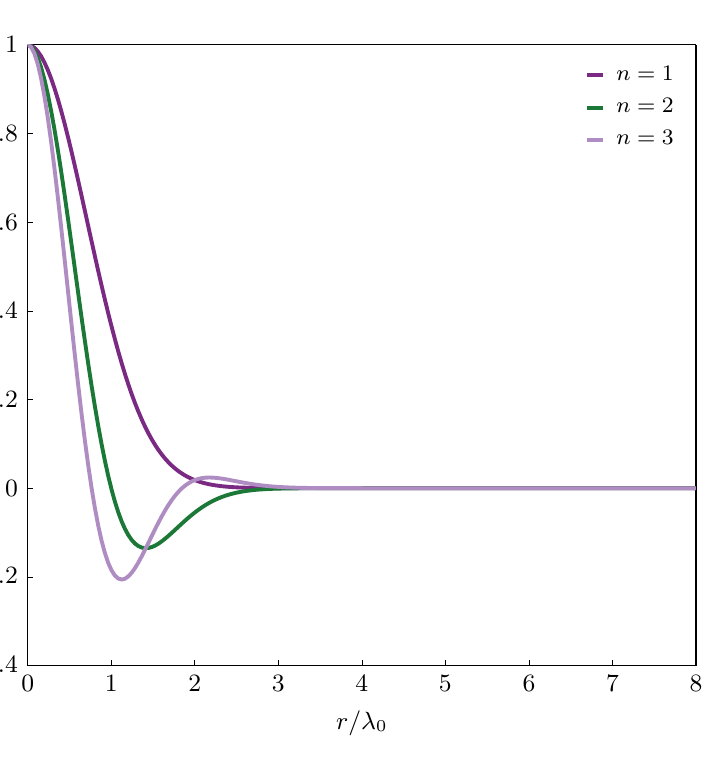
\begin{tikzpicture}[trim axis left,trim axis right]

\begin{axis}[%
width=11.252in,
height=7.131in,
at={(1.887in,0.962in)},
scale only axis,
clip=true,
separate axis lines,
every outer x axis line/.append style={black},
every x tick label/.append style={font=\color{black}},
every x tick/.append style={black},
xmin=0,
xmax=8,
xlabel={$r/\lambda_0$},
every outer y axis line/.append style={black},
every y tick label/.append style={font=\color{black}},
every y tick/.append style={black},
ymin=-0.4,
ymax=1,
ylabel={$C_{00,n}^{xy}(r)$},
axis background/.style={fill=white},
legend style={legend cell align=left, align=left},
clip=true,
clip mode=individual,
axis lines=box,
xtick pos=bottom,
ytick pos=left,
tick align=inside,
major tick length=2pt,
width=0.7\linewidth,
height=0.65\linewidth,
every axis/.append style={font=\fontsize{9}{9}\selectfont},xlabel style={font=\fontsize{9}{9}\selectfont},title style={font=\fontsize{9}{9}\selectfont},
legend style={font=\fontsize{8}{9}\selectfont,inner sep=1pt,row sep=1pt,column sep=2pt,nodes={scale=1.00},draw=none},legend image post style={xscale=0.35},
legend columns=1,
scaled x ticks=false,
tick label style={/pgf/number format/fixed,/pgf/number format/precision=2},
every x tick label/.append style={font=\fontsize{9}{9}\selectfont\color{black}},
every y tick label/.append style={font=\fontsize{9}{9}\selectfont\color{black}},
,,
colormap={sigmamap}{rgb(0.0000)=(0.0200,0.1880,0.3800); rgb(0.1000)=(0.0743,0.3456,0.5616); rgb(0.2000)=(0.1918,0.4980,0.7060); rgb(0.3000)=(0.3890,0.6708,0.8226); rgb(0.4000)=(0.7552,0.8682,0.9228); rgb(0.5000)=(0.9690,0.9689,0.9689); rgb(0.6000)=(0.9425,0.8044,0.7614); rgb(0.7000)=(0.8767,0.4910,0.4020); rgb(0.8000)=(0.7869,0.2866,0.2470); rgb(0.9000)=(0.6186,0.1239,0.1568); rgb(1.0000)=(0.4040,0.0000,0.1220)}
]
\addplot [color=mycolor1, line width=1.4pt]
  table[row sep=crcr]{%
1e-06	0.999999999999\\
0.0400210050025012	0.998399601164802\\
0.0800410100050025	0.993613914988808\\
0.120061015007504	0.985688746313652\\
0.160081020010005	0.974699624420412\\
0.200101025012506	0.960750604625268\\
0.240121030015008	0.943972627966267\\
0.280141035017509	0.924521475140297\\
0.32016104002001	0.902575359394744\\
0.360181045022511	0.878332210368438\\
0.400201050025012	0.852006706724764\\
0.440221055027514	0.823827119687516\\
0.484243060530265	0.79097308236634\\
0.524263065532766	0.759684729113178\\
0.564283070535268	0.727300616844434\\
0.604303075537769	0.6940701748391\\
0.64432308054027	0.660239763357353\\
0.684343085542771	0.626049737144811\\
0.724363090545273	0.59173174103289\\
0.764383095547774	0.557506276865767\\
0.804403100550275	0.523580573109958\\
0.844423105552776	0.490146780255911\\
0.884443110555278	0.457380506752258\\
0.924463115557779	0.425439701962636\\
0.96448312056028	0.39446388472475\\
1.00450312556278	0.364573708720333\\
1.04452313056528	0.335870849201984\\
1.08454313556778	0.308438189804935\\
1.12456314057028	0.282340283299189\\
1.16458314557279	0.257624056274803\\
1.20460315057529	0.234319724928809\\
1.24462315557779	0.212441887331191\\
1.28464316058029	0.191990756752799\\
1.32466316558279	0.172953500776418\\
1.36868517108554	0.153616030642925\\
1.40870517608804	0.137456156692945\\
1.44872518109055	0.122602894026061\\
1.48874518609305	0.109004923383705\\
1.52876519109555	0.096605170968143\\
1.56878519609805	0.0853421343566971\\
1.60880520110055	0.0751511263337177\\
1.64882520610305	0.0659654235207782\\
1.68884521110555	0.0577173101953688\\
1.72886521610805	0.0503390110203401\\
1.76888522111056	0.0437635094916467\\
1.80890522611306	0.0379252516972433\\
1.84892523111556	0.0327607374274328\\
1.88894523611806	0.0282090027635224\\
1.92896524112056	0.0242119999879278\\
1.96898524612306	0.0207148820077474\\
2.00900525112556	0.0176661994786927\\
2.04902525612806	0.0150180194791661\\
2.08904526113057	0.012725974944051\\
2.12906526613307	0.0107492541581323\\
2.16908527113557	0.00905053946678608\\
2.20910527613807	0.00759590402492638\\
2.25312728164082	0.00624120162348047\\
2.29314728664332	0.00520297616216849\\
2.33316729164582	0.00432358823816512\\
2.37318729664832	0.00358134108139998\\
2.41320730165083	0.00295703121831066\\
2.45322730665333	0.0024337446047919\\
2.49324731165583	0.00199665468359556\\
2.53326731665833	0.00163282555159215\\
2.57328732166083	0.00133102275996024\\
2.61330732666333	0.00108153366651469\\
2.65332733166583	0.000875998719344083\\
2.69334733666833	0.000707254577226614\\
2.73336734167084	0.000569189565086317\\
2.77338734667334	0.000456611620243819\\
2.81340735167584	0.000365128604090978\\
2.85342735667834	0.000291040629623266\\
2.89344736168084	0.000231243882767755\\
2.93346736668334	0.000183145288956025\\
2.97348737168584	0.000144587290025496\\
3.01350737668834	0.000113781944435656\\
3.05352738169085	8.92535403114787e-05\\
3.09354738669335	6.97889106716043e-05\\
3.1375693921961	5.3046498924736e-05\\
3.1775893971986	4.1199914486186e-05\\
3.2176094022011	3.18966278072457e-05\\
3.2576294072036	2.46151277540626e-05\\
3.2976494122061	1.89351297201011e-05\\
3.3376694172086	1.45192218940205e-05\\
3.37768942221111	1.1097554015231e-05\\
3.41770942721361	8.45512553019439e-06\\
3.45772943221611	6.42128164882296e-06\\
3.49774943721861	4.8610741519019e-06\\
3.53776944222111	3.66818845661831e-06\\
3.57778944722361	2.75917915890061e-06\\
3.61780945222611	2.06879295846269e-06\\
3.65782945722861	1.54619058659399e-06\\
3.69784946223112	1.15190824727759e-06\\
3.73786946723362	8.55424368192136e-07\\
3.77788947223612	6.33219404399189e-07\\
3.81790947723862	4.6723533522549e-07\\
3.85792948224112	3.43657646102901e-07\\
3.89794948724362	2.51956292962435e-07\\
3.93796949224612	1.84133698326139e-07\\
3.97798949724862	1.34137500465833e-07\\
4.02201150275138	9.43196276680939e-08\\
4.06203150775388	6.82492105497248e-08\\
4.10205151275638	4.92268508511979e-08\\
4.14207151775888	3.53928342989794e-08\\
4.18209152276138	2.53651537421737e-08\\
4.22211152776388	1.8120430961328e-08\\
4.26213153276638	1.29035263483008e-08\\
4.30215153776888	9.1591921633164e-09\\
4.34217154277139	6.48059372303923e-09\\
4.38219154777389	4.57068496023989e-09\\
4.42221155277639	3.21333975834547e-09\\
4.46223155777889	2.25185734354156e-09\\
4.50225156278139	1.57301899928504e-09\\
4.54227156778389	1.09530716668187e-09\\
4.58229157278639	7.60233070441163e-10\\
4.62231157778889	5.2597663614046e-10\\
4.6623315827914	3.6273963865497e-10\\
4.7023515877939	2.49363247995418e-10\\
4.7423715927964	1.70875084877425e-10\\
4.7823915977989	1.16716943962175e-10\\
4.8224116028014	7.9469035013004e-11\\
4.8624316078039	5.39350192834225e-11\\
4.90645361330665	3.50836095281114e-11\\
4.94647361830916	2.36513420422409e-11\\
4.98649362331166	1.58933766667526e-11\\
5.02651362831416	1.06459747216356e-11\\
5.06653363331666	7.1082640536508e-12\\
5.10655363831916	4.73097378204817e-12\\
5.14657364332166	3.13867535609458e-12\\
5.18659364832416	2.07563564786554e-12\\
5.22661365332666	1.36824765173743e-12\\
5.26663365832917	8.99056880984078e-13\\
5.30665366333167	5.88868731658669e-13\\
5.34667366833417	3.84466661568461e-13\\
5.38669367333667	2.50211776318582e-13\\
5.42671367833917	1.62317622470872e-13\\
5.46673368334167	1.04962089263502e-13\\
5.50675368834417	6.76562820137053e-14\\
5.54677369334667	4.34703018874741e-14\\
5.58679369834918	2.78410783066888e-14\\
5.62681370335168	1.77741284597066e-14\\
5.66683370835418	1.13109594300301e-14\\
5.70685371335668	7.17495930073217e-15\\
5.74687371835918	4.53678612841743e-15\\
5.79089572386193	2.73000409792804e-15\\
5.83091572886443	1.71463144696031e-15\\
5.87093573386693	1.07346314241637e-15\\
5.91095573886944	6.69903670730517e-16\\
5.95097574387194	4.1672201538937e-16\\
5.99099574887444	2.58398149592029e-16\\
6.03101575387694	1.59713350705079e-16\\
6.07103575887944	9.84015433414923e-17\\
6.11105576388194	6.04326259970597e-17\\
6.15107576888444	3.69955841911029e-17\\
6.19109577388694	2.25754897281505e-17\\
6.23111577888945	1.37319855590568e-17\\
6.27113578389195	8.32603750963023e-18\\
6.31115578889445	5.03213467220562e-18\\
6.35117579389695	3.03162175470186e-18\\
6.39119579889945	1.82056689621065e-18\\
6.43121580390195	1.08980083300828e-18\\
6.47123580890445	6.50274159901648e-19\\
6.51125581390695	3.86771731816392e-19\\
6.55127581890946	2.29309380300723e-19\\
6.59129582391196	1.35518249587828e-19\\
6.63131582891446	7.98330301173825e-20\\
6.67533783441721	4.44405237063416e-20\\
6.71535783941971	2.60041474190959e-20\\
6.75537784442221	1.51675326273018e-20\\
6.79539784942471	8.81852851361355e-21\\
6.83541785442721	5.11076811135279e-21\\
6.87543785942972	2.95246730096635e-21\\
6.91545786443222	1.70017209473838e-21\\
6.95547786943472	9.75909483367566e-22\\
6.99549787443722	5.5838669301376e-22\\
7.03551787943972	3.18470675439909e-22\\
7.07553788444222	1.81055909834295e-22\\
7.11555788944472	1.02604126765943e-22\\
7.15557789444722	5.79596586689341e-23\\
7.19559789944972	3.2635906260576e-23\\
7.23561790445223	1.83178459397958e-23\\
7.27563790945473	1.02485398559846e-23\\
7.31565791445723	5.71555560072707e-24\\
7.35567791945973	3.17734066173813e-24\\
7.39569792446223	1.76067004143708e-24\\
7.43571792946473	9.72525585628352e-25\\
7.47573793446723	5.35467311999438e-25\\
7.51575793946973	2.93882523083718e-25\\
7.55977994497249	1.51339354258516e-25\\
7.59979994997499	8.2503294939145e-26\\
7.63981995497749	4.48331834106133e-26\\
7.67983995997999	2.4284922874267e-26\\
7.71985996498249	1.31124168431141e-26\\
7.75987996998499	7.05728461628706e-27\\
7.79989997498749	3.78618111991713e-27\\
7.83991997999	2.02476211218377e-27\\
7.8799399849925	1.07933309282375e-27\\
7.919959989995	5.73516408144493e-28\\
7.9599799949975	3.0377013151799e-28\\
8	1.60381089054864e-28\\
};
\addlegendentry{$n=1$}

\addplot [color=mycolor2, line width=1.4pt]
  table[row sep=crcr]{%
1e-06	0.999999999998\\
0.0400210050025012	0.996800483651545\\
0.0800410100050025	0.98724826456394\\
0.120061015007504	0.971480390663682\\
0.160081020010005	0.949722037181622\\
0.200101025012506	0.922281746698046\\
0.240121030015008	0.889544951237612\\
0.280141035017509	0.851965954754393\\
0.32016104002001	0.810058594702914\\
0.360181045022511	0.764385834389475\\
0.400201050025012	0.715548562433984\\
0.440221055027514	0.664173891268017\\
0.484243060530265	0.605496743056042\\
0.524263065532766	0.550884042841713\\
0.564283070535268	0.495716911871969\\
0.604303075537769	0.440608096506016\\
0.64432308054027	0.386139751867212\\
0.684343085542771	0.332854706808546\\
0.724363090545273	0.281248979948098\\
0.764383095547774	0.231765663815864\\
0.804403100550275	0.184790250853524\\
0.844423105552776	0.140647431754698\\
0.884443110555278	0.0995993548719855\\
0.924463115557779	0.0618452964606401\\
0.96448312056028	0.0275226565096869\\
1.00450312556278	-0.00329083525115842\\
1.04452313056528	-0.0305738432035671\\
1.08454313556778	-0.0543572382355185\\
1.12456314057028	-0.0747191698508242\\
1.16458314557279	-0.0917795755422772\\
1.20460315057529	-0.105694305512064\\
1.24462315557779	-0.116649035973267\\
1.28464316058029	-0.124853134646875\\
1.32466316558279	-0.130533628414198\\
1.36868517108554	-0.134152740929596\\
1.40870517608804	-0.135318751000766\\
1.44872518109055	-0.134716630099241\\
1.48874518609305	-0.132589471591537\\
1.52876519109555	-0.129172996938708\\
1.56878519609805	-0.124692282335108\\
1.60880520110055	-0.119359090162107\\
1.64882520610305	-0.113369796992132\\
1.68884521110555	-0.106903894997967\\
1.72886521610805	-0.100123031195721\\
1.76888522111056	-0.0931705390878027\\
1.80890522611306	-0.0861714099803679\\
1.84892523111556	-0.0792326464422981\\
1.88894523611806	-0.0724439378864841\\
1.92896524112056	-0.0658785978650915\\
1.96898524612306	-0.0595947041098592\\
2.00900525112556	-0.0536363853194966\\
2.04902525612806	-0.0480352028889651\\
2.08904526113057	-0.0428115808804694\\
2.12906526613307	-0.0379762432562971\\
2.16908527113557	-0.0335316234539607\\
2.20910527613807	-0.0294732175382701\\
2.25312728164082	-0.0254427736122996\\
2.29314728664332	-0.0221570013462918\\
2.33316729164582	-0.0192125976635722\\
2.37318729664832	-0.0165888361561136\\
2.41320730165083	-0.0142634455382412\\
2.45322730665333	-0.0122133194909206\\
2.49324731165583	-0.0104151141998878\\
2.53326731665833	-0.00884573984070343\\
2.57328732166083	-0.00748275392071925\\
2.61330732666333	-0.00630466551580028\\
2.65332733166583	-0.00529116009842465\\
2.69334733666833	-0.00442325490878138\\
2.73336734167084	-0.00368339473892676\\
2.77338734667334	-0.00305549764820509\\
2.81340735167584	-0.00252495956900456\\
2.85342735667834	-0.00207862605354012\\
2.89344736168084	-0.00170473860658529\\
2.93346736668334	-0.0013928621908675\\
2.97348737168584	-0.00113379961894743\\
3.01350737668834	-0.000919497688415777\\
3.05352738169085	-0.00074294909992025\\
3.09354738669335	-0.000598093437336176\\
3.1375693921961	-0.000469161361993449\\
3.1775893971986	-0.000374798686414659\\
3.2176094022011	-0.000298329487304294\\
3.2576294072036	-0.000236604284356521\\
3.2976494122061	-0.000186974780233718\\
3.3376694172086	-0.000147225449228501\\
3.37768942221111	-0.000115512063013765\\
3.41770942721361	-9.03069782526349e-05\\
3.45772943221611	-7.03508735527202e-05\\
3.49774943721861	-5.46105277624496e-05\\
3.53776944222111	-4.22421709444225e-05\\
3.57778944722361	-3.25599070282465e-05\\
3.61780945222611	-2.50086972552949e-05\\
3.65782945722861	-1.91414008667813e-05\\
3.69784946223112	-1.45993895410912e-05\\
3.73786946723362	-1.10962810350996e-05\\
3.77788947223612	-8.40437216485464e-06\\
3.81790947723862	-6.34338911944219e-06\\
3.85792948224112	-4.77121213076601e-06\\
3.89794948724362	-3.57627019354867e-06\\
3.93796949224612	-2.67133872715635e-06\\
3.97798949724862	-1.98850802095575e-06\\
4.02201150275138	-1.43144904742223e-06\\
4.06203150775388	-1.05786958639331e-06\\
4.10205151275638	-7.79104833141027e-07\\
4.14207151775888	-5.71833404135077e-07\\
4.18209152276138	-4.18268582479506e-07\\
4.22211152776388	-3.04898462094721e-07\\
4.26213153276638	-2.21498903580513e-07\\
4.30215153776888	-1.60363787927053e-07\\
4.34217154277139	-1.1570746062093e-07\\
4.38219154777389	-8.3202933363625e-08\\
4.42221155277639	-5.96265880118317e-08\\
4.46223155777889	-4.25860237411274e-08\\
4.50225156278139	-3.03124994700107e-08\\
4.54227156778389	-2.15033233073229e-08\\
4.58229157278639	-1.52026818060235e-08\\
4.62231157778889	-1.07119162105998e-08\\
4.6623315827914	-7.52225369036748e-09\\
4.7023515877939	-5.26458443515363e-09\\
4.7423715927964	-3.67212066641458e-09\\
4.7823915977989	-2.55274772432255e-09\\
4.8224116028014	-1.76863532048689e-09\\
4.8624316078039	-1.22126364755585e-09\\
4.90645361330665	-8.09494193726573e-10\\
4.94647361830916	-5.55040264231443e-10\\
4.98649362331166	-3.7929731998587e-10\\
5.02651362831416	-2.58333511314688e-10\\
5.06653363331666	-1.75359189953915e-10\\
5.10655363831916	-1.1863810941404e-10\\
5.14657364332166	-7.99961101446666e-11\\
5.18659364832416	-5.37605276299237e-11\\
5.22661365332666	-3.60088442767934e-11\\
5.26663365832917	-2.40384705031853e-11\\
5.30665366333167	-1.5994012234022e-11\\
5.34667366833417	-1.06062507722495e-11\\
5.38669367333667	-7.0100504071987e-12\\
5.42671367833917	-4.61780997013962e-12\\
5.46673368334167	-3.03184854394097e-12\\
5.50675368834417	-1.98397555873564e-12\\
5.54677369334667	-1.29396736586755e-12\\
5.58679369834918	-8.41142003055296e-13\\
5.62681370335168	-5.44973129513101e-13\\
5.66683370835418	-3.51917929136384e-13\\
5.70685371335668	-2.26500401716275e-13\\
5.74687371835918	-1.45297641964696e-13\\
5.79089572386193	-8.8819245391004e-14\\
5.83091572886443	-5.65821145817908e-14\\
5.87093573386693	-3.59265424955271e-14\\
5.91095573886944	-2.27361271330136e-14\\
5.95097574387194	-1.43411182372224e-14\\
5.99099574887444	-9.0160360037968e-15\\
6.03101575387694	-5.64956447496186e-15\\
6.07103575887944	-3.5284308985916e-15\\
6.11105576388194	-2.1964239459225e-15\\
6.15107576888444	-1.3627594656806e-15\\
6.19109577388694	-8.42735511237248e-16\\
6.23111577888945	-5.19437124212444e-16\\
6.27113578389195	-3.19113238747604e-16\\
6.31115578889445	-1.95401248369331e-16\\
6.35117579389695	-1.19256220582389e-16\\
6.39119579889945	-7.25448277374096e-17\\
6.43121580390195	-4.39849465341486e-17\\
6.47123580890445	-2.65811871863263e-17\\
6.51125581390695	-1.60109775371226e-17\\
6.55127581890946	-9.61246918119099e-18\\
6.59129582391196	-5.7520965835442e-18\\
6.63131582891446	-3.43077254771283e-18\\
6.67533783441721	-1.93583522116711e-18\\
6.71535783941971	-1.1466796884185e-18\\
6.75537784442221	-6.7700478788251e-19\\
6.79539784942471	-3.98398471663878e-19\\
6.83541785442721	-2.33679329627201e-19\\
6.87543785942972	-1.3661552106499e-19\\
6.91545786443222	-7.9608105794927e-20\\
6.95547786943472	-4.62372956969093e-20\\
6.99549787443722	-2.6767377604612e-20\\
7.03551787943972	-1.54453538209407e-20\\
7.07553788444222	-8.8831888975206e-21\\
7.11555788944472	-5.09236225060441e-21\\
7.15557789444722	-2.9097078828001e-21\\
7.19559789944972	-1.65714130853316e-21\\
7.23561790445223	-9.40697709566797e-22\\
7.27563790945473	-5.3225696419869e-22\\
7.31565791445723	-3.00174411384222e-22\\
7.35567791945973	-1.68735845730853e-22\\
7.39569792446223	-9.45415508882542e-23\\
7.43571792946473	-5.27983178868163e-23\\
7.47573793446723	-2.93900110444211e-23\\
7.51575793946973	-1.63065471202749e-23\\
7.55977994497249	-8.49774602947474e-24\\
7.59979994997499	-4.68263615129716e-24\\
7.63981995497749	-2.57193846041647e-24\\
7.67983995997999	-1.40803841513233e-24\\
7.71985996498249	-7.68338296506925e-25\\
7.75987996998499	-4.17902310820732e-25\\
7.79989997498749	-2.26559170333825e-25\\
7.83991997999	-1.22425915486547e-25\\
7.8799399849925	-6.59401868374441e-26\\
7.919959989995	-3.54007397457217e-26\\
7.9599799949975	-1.89434946891918e-26\\
8	-1.01040086104564e-26\\
};
\addlegendentry{$n=2$}

\addplot [color=mycolor3, line width=1.4pt]
  table[row sep=crcr]{%
1e-06	0.999999999997\\
0.0400210050025012	0.99520264677623\\
0.0800410100050025	0.980903005110212\\
0.120061015007504	0.957374439231591\\
0.160081020010005	0.925064486930967\\
0.200101025012506	0.884583043389047\\
0.240121030015008	0.836686372969184\\
0.280141035017509	0.782257476692557\\
0.32016104002001	0.722283457211489\\
0.360181045022511	0.65783061203409\\
0.400201050025012	0.590018046409692\\
0.440221055027514	0.519990627805751\\
0.484243060530265	0.44176670157236\\
0.524263065532766	0.37077797482217\\
0.564283070535268	0.301003114037397\\
0.604303075537769	0.233425938764405\\
0.64432308054027	0.168936356173771\\
0.684343085542771	0.108315025012104\\
0.724363090545273	0.0522216641657382\\
0.764383095547774	0.0011871604973946\\
0.804403100550275	-0.0443905018834978\\
0.844423105552776	-0.0842465949090469\\
0.884443110555278	-0.118246501613079\\
0.924463115557779	-0.146379392601539\\
0.96448312056028	-0.168749126189556\\
1.00450312556278	-0.185562837200974\\
1.04452313056528	-0.197117721187076\\
1.08454313556778	-0.203786541461311\\
1.12456314057028	-0.206002386620344\\
1.16458314557279	-0.204243187680562\\
1.20460315057529	-0.199016468821881\\
1.24462315557779	-0.19084475673101\\
1.28464316058029	-0.180252013757371\\
1.32466316558279	-0.167751392801878\\
1.36868517108554	-0.152383022457257\\
1.40870517608804	-0.137439538655591\\
1.44872518109055	-0.122004447297636\\
1.48874518609305	-0.106453520672244\\
1.52876519109555	-0.0911154892160205\\
1.56878519609805	-0.0762702136835455\\
1.60880520110055	-0.0621483666866192\\
1.64882520610305	-0.0489324500001596\\
1.68884521110555	-0.0367589519805289\\
1.72886521610805	-0.0257214369501888\\
1.76888522111056	-0.0158743547841\\
1.80890522611306	-0.00723736322042795\\
1.84892523111556	0.00020003356054727\\
1.88894523611806	0.00647371008769024\\
1.92896524112056	0.0116401679354758\\
1.96898524612306	0.0157719434090352\\
2.00900525112556	0.0189532859681485\\
2.04902525612806	0.0212761936768565\\
2.08904526113057	0.0228368675313141\\
2.12906526613307	0.023732623581764\\
2.16908527113557	0.0240592809691401\\
2.20910527613807	0.0239090258024204\\
2.25312728164082	0.0232964090070341\\
2.29314728664332	0.02241957687141\\
2.33316729164582	0.0213128264084734\\
2.37318729664832	0.0200403866838539\\
2.41320730165083	0.0186583991468383\\
2.45322730665333	0.0172150066990815\\
2.49324731165583	0.0157506456407219\\
2.53326731665833	0.0142984943898845\\
2.57328732166083	0.0128850362784983\\
2.61330732666333	0.0115306980002704\\
2.65332733166583	0.010250530105904\\
2.69334733666833	0.0090549010232812\\
2.73336734167084	0.0079501811855913\\
2.77338734667334	0.00693939878212585\\
2.81340735167584	0.00602285325316882\\
2.85342735667834	0.00519867682311919\\
2.89344736168084	0.00446333803466766\\
2.93346736668334	0.00381208437573296\\
2.97348737168584	0.00323932367309791\\
3.01350737668834	0.0027389459787743\\
3.05352738169085	0.00230458923142039\\
3.09354738669335	0.0019298530826504\\
3.1375693921961	0.00157902708535051\\
3.1775893971986	0.00130938711973568\\
3.2176094022011	0.00108086157736653\\
3.2576294072036	0.000888226011362204\\
3.2976494122061	0.000726698107604974\\
3.3376694172086	0.000591950701284288\\
3.37768942221111	0.000480109322492955\\
3.41770942721361	0.000387738033883611\\
3.45772943221611	0.000311816801066955\\
3.49774943721861	0.000249713126653047\\
3.53776944222111	0.000199150197589604\\
3.57778944722361	0.00015817335374278\\
3.61780945222611	0.000125116290255197\\
3.65782945722861	9.85680603628926e-05\\
3.69784946223112	7.73416495403549e-05\\
3.73786946723362	6.04446444466514e-05\\
3.77788947223612	4.70523180307922e-05\\
3.81790947723862	3.64832911902355e-05\\
3.85792948224112	2.8177806865108e-05\\
3.89794948724362	2.16785594716875e-05\\
3.93796949224612	1.66139562539033e-05\\
3.97798949724862	1.26836428194304e-05\\
4.02201150275138	9.38363914600103e-06\\
4.06203150775388	7.10654798048342e-06\\
4.10205151275638	5.36166029528959e-06\\
4.14207151775888	4.02995670136077e-06\\
4.18209152276138	3.01765019484769e-06\\
4.22211152776388	2.25118649987996e-06\\
4.26213153276638	1.67314841899372e-06\\
4.30215153776888	1.23892193619445e-06\\
4.34217154277139	9.13998992114544e-07\\
4.38219154777389	6.71808297922792e-07\\
4.42221155277639	4.91980884606539e-07\\
4.46223155777889	3.5897106462663e-07\\
4.50225156278139	2.60966002494617e-07\\
4.54227156778389	1.89028128279455e-07\\
4.58229157278639	1.3642422626838e-07\\
4.62231157778889	9.8103275963237e-08\\
4.6623315827914	7.02921268197431e-08\\
4.7023515877939	5.01839779887669e-08\\
4.7423715927964	3.56995405202621e-08\\
4.7823915977989	2.53048103913761e-08\\
4.8224116028014	1.78726977398493e-08\\
4.8624316078039	1.25784524767123e-08\\
4.90645361330665	8.51180995394734e-09\\
4.94647361830916	5.94586586592604e-09\\
4.98649362331166	4.13874376523606e-09\\
5.02651362831416	2.87068323127658e-09\\
5.06653363331666	1.9841215110809e-09\\
5.10655363831916	1.36653381710714e-09\\
5.14657364332166	9.37873792022771e-10\\
5.18659364832416	6.41420746278332e-10\\
5.22661365332666	4.37138236542148e-10\\
5.26663365832917	2.96875463343613e-10\\
5.30665366333167	2.00914822642777e-10\\
5.34667366833417	1.35498408044807e-10\\
5.38669367333667	9.10632727204254e-11\\
5.42671367833917	6.09875802073137e-11\\
5.46673368334167	4.07034115753854e-11\\
5.50675368834417	2.70715794329505e-11\\
5.54677369334667	1.79428656461657e-11\\
5.58679369834918	1.18513395143147e-11\\
5.62681370335168	7.80085921105328e-12\\
5.66683370835418	5.1170386085357e-12\\
5.70685371335668	3.34501476572425e-12\\
5.74687371835918	2.17912560999528e-12\\
5.79089572386193	1.35465943572789e-12\\
5.83091572886443	8.76153528176437e-13\\
5.87093573386693	5.64729447267646e-13\\
5.91095573886944	3.62754152027037e-13\\
5.95097574387194	2.32218947546531e-13\\
5.99099574887444	1.48148664568334e-13\\
6.03101575387694	9.41920275446321e-14\\
6.07103575887944	5.96826800249013e-14\\
6.11105576388194	3.76878766979996e-14\\
6.15107576888444	2.37178647307976e-14\\
6.19109577388694	1.48754946957223e-14\\
6.23111577888945	9.29801998798465e-15\\
6.27113578389195	5.79207327258321e-15\\
6.31115578889445	3.59586507998287e-15\\
6.35117579389695	2.22484481957682e-15\\
6.39119579889945	1.37190568341215e-15\\
6.43121580390195	8.43098177828627e-16\\
6.47123580890445	5.1637184654508e-16\\
6.51125581390695	3.15194470335858e-16\\
6.55127581890946	1.9174645657742e-16\\
6.59129582391196	1.16254533560458e-16\\
6.63131582891446	7.02469204081058e-17\\
6.67533783441721	4.02045664999467e-17\\
6.71535783941971	2.41223297308923e-17\\
6.75537784442221	1.44245097440607e-17\\
6.79539784942471	8.59650218177638e-18\\
6.83541785442721	5.10601794827208e-18\\
6.87543785942972	3.02262074322651e-18\\
6.91545786443222	1.78330916672957e-18\\
6.95547786943472	1.04860559212389e-18\\
6.99549787443722	6.14527192170623e-19\\
7.03551787943972	3.58933748357849e-19\\
7.07553788444222	2.0894528137649e-19\\
7.11555788944472	1.21226268888292e-19\\
7.15557789444722	7.0098319041038e-20\\
7.19559789944972	4.03985655585005e-20\\
7.23561790445223	2.3204516749918e-20\\
7.27563790945473	1.32839767309582e-20\\
7.31565791445723	7.57937536174555e-21\\
7.35567791945973	4.31011819777227e-21\\
7.39569792446223	2.4428461126369e-21\\
7.43571792946473	1.37992314818243e-21\\
7.47573793446723	7.76901992779973e-22\\
7.51575793946973	4.35944082245404e-22\\
7.55977994497249	2.30001963233174e-22\\
7.59979994997499	1.28162206881505e-22\\
7.63981995497749	7.11776475244733e-23\\
7.67983995997999	3.93988118118765e-23\\
7.71985996498249	2.1735972291881e-23\\
7.75987996998499	1.19517657425422e-23\\
7.79989997498749	6.55002135627364e-24\\
7.83991997999	3.57776311683082e-24\\
7.8799399849925	1.9477770377773e-24\\
7.919959989995	1.05688139523921e-24\\
7.9599799949975	5.71574922894909e-25\\
8	3.08092072074393e-25\\
};
\addlegendentry{$n=3$}

\node[overlay,right, align=left, inner sep=0]
at (rel axis cs:-0.15,1.1) {$(a)$};
\end{axis}
\end{tikzpicture}%
  %% This file was created by matlab2tikz.
%
\definecolor{mycolor1}{rgb}{0.48200,0.16500,0.51400}%
\definecolor{mycolor2}{rgb}{0.10600,0.47100,0.21600}%
\definecolor{mycolor3}{rgb}{0.68600,0.55300,0.76500}%
%
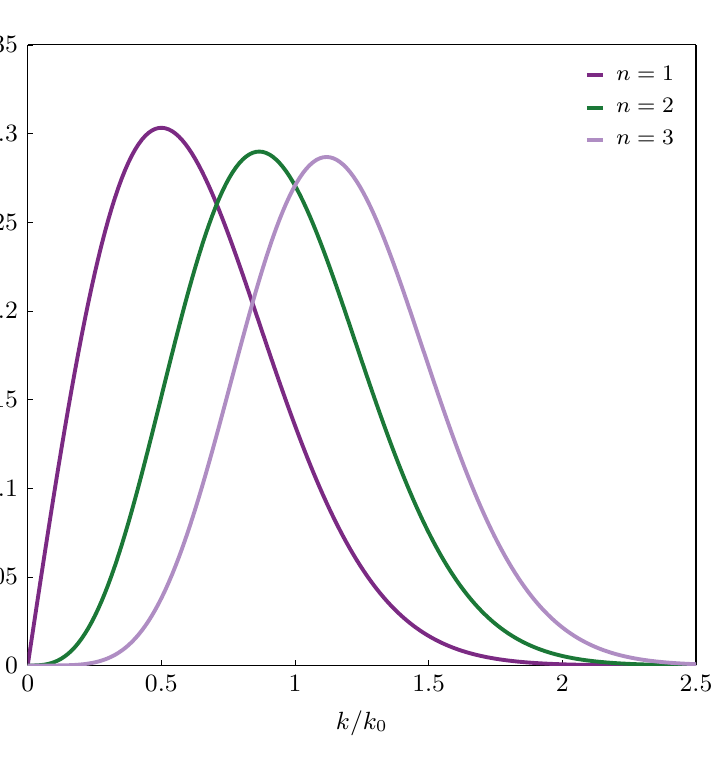
\begin{tikzpicture}[trim axis left,trim axis right]

\begin{axis}[%
width=11.252in,
height=7.131in,
at={(1.887in,0.962in)},
scale only axis,
clip=true,
separate axis lines,
every outer x axis line/.append style={black},
every x tick label/.append style={font=\color{black}},
every x tick/.append style={black},
xmin=0,
xmax=2.5,
xlabel={$k/k_0$},
every outer y axis line/.append style={black},
every y tick label/.append style={font=\color{black}},
every y tick/.append style={black},
ymin=0,
ymax=0.35,
ylabel={$E_{\eta,n}(k)$},
axis background/.style={fill=white},
legend style={legend cell align=left, align=left},
clip=true,
clip mode=individual,
axis lines=box,
xtick pos=bottom,
ytick pos=left,
tick align=inside,
major tick length=2pt,
width=0.7\linewidth,
height=0.65\linewidth,
every axis/.append style={font=\fontsize{9}{9}\selectfont},xlabel style={font=\fontsize{9}{9}\selectfont},title style={font=\fontsize{9}{9}\selectfont},
legend style={font=\fontsize{8}{9}\selectfont,inner sep=1pt,row sep=1pt,column sep=2pt,nodes={scale=1.00},draw=none},legend image post style={xscale=0.35},
legend columns=1,
scaled x ticks=false,
tick label style={/pgf/number format/fixed,/pgf/number format/precision=2},
every x tick label/.append style={font=\fontsize{9}{9}\selectfont\color{black}},
every y tick label/.append style={font=\fontsize{9}{9}\selectfont\color{black}},
,,
colormap={sigmamap}{rgb(0.0000)=(0.0200,0.1880,0.3800); rgb(0.1000)=(0.0743,0.3456,0.5616); rgb(0.2000)=(0.1918,0.4980,0.7060); rgb(0.3000)=(0.3890,0.6708,0.8226); rgb(0.4000)=(0.7552,0.8682,0.9228); rgb(0.5000)=(0.9690,0.9689,0.9689); rgb(0.6000)=(0.9425,0.8044,0.7614); rgb(0.7000)=(0.8767,0.4910,0.4020); rgb(0.8000)=(0.7869,0.2866,0.2470); rgb(0.9000)=(0.6186,0.1239,0.1568); rgb(1.0000)=(0.4040,0.0000,0.1220)}
]
\addplot [color=mycolor1, line width=1.4pt]
  table[row sep=crcr]{%
1e-06	9.99999999998e-07\\
0.012507248124062	0.0125033356870642\\
0.0250134962481241	0.0249822151857268\\
0.0375197443721861	0.0374142575081492\\
0.0500259924962481	0.049776227988151\\
0.0625322406203102	0.0620451106388611\\
0.0750384887443722	0.074198179555138\\
0.0875447368684342	0.0862130690507178\\
0.100050984992496	0.0980678422271457\\
0.112557233116558	0.109741057680322\\
0.12506348124062	0.121211834060891\\
0.137569729364682	0.132459912216648\\
0.151326602301151	0.144552237739127\\
0.163832850425213	0.15526980755966\\
0.176339098549275	0.165706455442367\\
0.188845346673337	0.175845062145538\\
0.201351594797399	0.185669401013813\\
0.213857842921461	0.195164180365556\\
0.226364091045523	0.204315081990821\\
0.238870339169585	0.213108795630047\\
0.251376587293647	0.221533049324865\\
0.263882835417709	0.229576635554121\\
0.276389083541771	0.237229433090159\\
0.288895331665833	0.244482424532426\\
0.301401579789895	0.251327709497517\\
0.313907827913957	0.257758513466586\\
0.326414076038019	0.26376919231265\\
0.338920324162081	0.269355232551407\\
0.351426572286143	0.274513247379763\\
0.363932820410205	0.279240968586193\\
0.376439068534267	0.283537234436133\\
0.388945316658329	0.287401973653864\\
0.401451564782391	0.290836185639548\\
0.413957812906453	0.293841917076269\\
0.427714685842921	0.296657016968592\\
0.440220933966983	0.298774103791276\\
0.452727182091046	0.300475402147823\\
0.465233430215107	0.301766937984341\\
0.47773967833917	0.302655615812989\\
0.490245926463232	0.303149177432573\\
0.502752174587294	0.303256158493771\\
0.515258422711356	0.302985843147067\\
0.527764670835418	0.302348217015337\\
0.54027091895948	0.30135391873543\\
0.552777167083542	0.300014190314105\\
0.565283415207604	0.298340826543286\\
0.577789663331666	0.296346123717858\\
0.590295911455728	0.2940428278962\\
0.60280215957979	0.291444082939338\\
0.615308407703852	0.288563378559127\\
0.627814655827914	0.285414498599276\\
0.640320903951976	0.282011469765338\\
0.652827152076038	0.278368511011214\\
0.6653334002001	0.274499983780127\\
0.677839648324162	0.270420343287768\\
0.690345896448224	0.266144091024213\\
0.704102769384692	0.261230433566072\\
0.716609017508754	0.256588445151956\\
0.729115265632816	0.251794604352604\\
0.741621513756878	0.24686313763554\\
0.75412776188094	0.241808100063135\\
0.766634010005002	0.23664333833741\\
0.779140258129065	0.231382455957741\\
0.791646506253126	0.226038780563521\\
0.804152754377189	0.220625333520528\\
0.816659002501251	0.215154801796455\\
0.829165250625313	0.209639512158135\\
0.841671498749375	0.204091407710348\\
0.854177746873437	0.19852202678381\\
0.866683994997499	0.192942484168157\\
0.879190243121561	0.187363454674395\\
0.891696491245623	0.181795159000548\\
0.904202739369685	0.176247351864029\\
0.916708987493747	0.170729312354729\\
0.929215235617809	0.165249836453935\\
0.941721483741871	0.159817231655987\\
0.954227731865933	0.154439313622079\\
0.966733979989995	0.149123404788854\\
0.980490852926463	0.143355662283408\\
0.992997101050525	0.138191618138487\\
1.00550334917459	0.13310916348621\\
1.01800959729865	0.128113622286538\\
1.03051584542271	0.123209845332416\\
1.04302209354677	0.11840221880887\\
1.05552834167084	0.113694674126555\\
1.0680345897949	0.109090698924165\\
1.08054083791896	0.104593349133712\\
1.09304708604302	0.100205262002926\\
1.10555333416708	0.0959286699697512\\
1.11805958229115	0.0917654152852739\\
1.13056583041521	0.0877169652831892\\
1.14307207853927	0.0837844281962175\\
1.15557832666333	0.0799685694225552\\
1.16808457478739	0.0762698281485362\\
1.18059082291146	0.0726883342371032\\
1.19309707103552	0.0692239252954183\\
1.20560331915958	0.0658761638389392\\
1.21810956728364	0.0626443544735069\\
1.2306158154077	0.0595275610214065\\
1.24312206353177	0.0565246235219153\\
1.25687893646823	0.0533512586932931\\
1.2693851845923	0.050582742554742\\
1.28189143271636	0.04792324446996\\
1.29439768084042	0.0453708597065667\\
1.30690392896448	0.0429235422940296\\
1.31941017708854	0.0405791200311605\\
1.33191642521261	0.038335309011414\\
1.34442267333667	0.0361897276348124\\
1.35692892146073	0.0341399100797784\\
1.36943516958479	0.0321833192124766\\
1.38194141770885	0.0303173589154311\\
1.39444766583292	0.028539385821176\\
1.40695391395698	0.0268467204405133\\
1.41946016208104	0.025236657678563\\
1.4319664102051	0.0237064767352062\\
1.44447265832916	0.022253450389725\\
1.45697890645323	0.020874853672428\\
1.46948515457729	0.0195679719288212\\
1.48199140270135	0.0183301082844277\\
1.49449765082541	0.0171585905206906\\
1.50700389894947	0.0160507773744975\\
1.51951014707354	0.015004064275758\\
1.53326702001	0.0139201932227356\\
1.54577326813407	0.0129935043648222\\
1.55827951625813	0.0121201276874942\\
1.57078576438219	0.0112976577428226\\
1.58329201250625	0.0105237469402583\\
1.59579826063032	0.0097961082518346\\
1.60830450875438	0.00911251749448843\\
1.62081075687844	0.00847081521196432\\
1.6333170050025	0.00786890817898354\\
1.64582325312656	0.00730477055043469\\
1.65832950125063	0.00677644467828962\\
1.67083574937469	0.00628204161877771\\
1.68334199749875	0.00581974135207076\\
1.69584824562281	0.00538779273635341\\
1.70835449374687	0.00498451321768748\\
1.72086074187094	0.00460828831653454\\
1.733366989995	0.00425757091118747\\
1.74587323811906	0.00393088033768892\\
1.75837948624312	0.00362680132509161\\
1.77088573436718	0.00334398278414903\\
1.78339198249125	0.00308113646672591\\
1.79589823061531	0.00283703551239094\\
1.80965510355178	0.0025887842603378\\
1.82216135167584	0.00238031932361065\\
1.8346675997999	0.00218716939922618\\
1.84717384792396	0.00200834229180101\\
1.85968009604802	0.00184289856882796\\
1.87218634417209	0.00168994972555733\\
1.88469259229615	0.00154865632932159\\
1.89719884042021	0.00141822615287879\\
1.90970508854427	0.00129791230555245\\
1.92221133666833	0.00118701137017154\\
1.9347175847924	0.00108486155306661\\
1.94722383291646	0.000990840853659224\\
1.95973008104052	0.000904365259492857\\
1.97223632916458	0.000824886971896154\\
1.98474257728864	0.000751892666844868\\
1.99724882541271	0.000684901794997244\\
2.00975507353677	0.00062346492432005\\
2.02226132166083	0.000567162128198694\\
2.03476756978489	0.000515601421434883\\
2.04727381790895	0.000468417246079032\\
2.05978006603302	0.000425269008621212\\
2.07228631415708	0.00038583966967374\\
2.08604318709355	0.000346411460523943\\
2.09854943521761	0.000313856995799808\\
2.11105568334167	0.000284173937835262\\
2.12356193146573	0.000257128211923276\\
2.13606817958979	0.000232502938143593\\
2.14857442771386	0.00021009734700092\\
2.16108067583792	0.000189725746983587\\
2.17358692396198	0.000171216543082732\\
2.18609317208604	0.000154411305167679\\
2.19859942021011	0.00013916388498924\\
2.21110566833417	0.000125339580478016\\
2.22361191645823	0.000112814345917912\\
2.23611816458229	0.000101474046504826\\
2.24862441270635	9.12137557453812e-05\\
2.26113066083042	8.19370941095129e-05\\
2.27363690895448	7.35556073223929e-05\\
2.28614315707854	6.59881826644289e-05\\
2.2986494052026	5.91605016418098e-05\\
2.31115565332666	5.30045273931476e-05\\
2.32366190145073	4.74580252092345e-05\\
2.33616814957479	4.2464114561786e-05\\
2.34867439769885	3.79708510623788e-05\\
2.36243127063532	3.35500659514266e-05\\
2.37493751875938	2.99588643141167e-05\\
2.38744376688344	2.67345922799202e-05\\
2.3999500150075	2.38417517501924e-05\\
2.41245626313157	2.12480587809647e-05\\
2.42496251125563	1.89241760545548e-05\\
2.43746875937969	1.68434651930235e-05\\
2.44997500750375	1.49817576851635e-05\\
2.46248125562781	1.33171432506067e-05\\
2.47498750375188	1.182977451687e-05\\
2.48749375187594	1.05016869373549e-05\\
2.5	9.31663293019668e-06\\
};
\addlegendentry{$n=1$}

\addplot [color=mycolor2, line width=1.4pt]
  table[row sep=crcr]{%
1e-06	1.999999999996e-18\\
0.012507248124062	3.91182500235304e-06\\
0.0250134962481241	3.12614947005987e-05\\
0.0375197443721861	0.000105338436566632\\
0.0500259924962481	0.000249139968883221\\
0.0625322406203102	0.000485227649066178\\
0.0750384887443722	0.000835586478256945\\
0.0875447368684342	0.00132148788088522\\
0.100050984992496	0.00196335734967166\\
0.112557233116558	0.00278064761171072\\
0.12506348124062	0.00379171813014021\\
0.137569729364682	0.00501372170881961\\
0.151326602301151	0.00662041748434639\\
0.163832850425213	0.00833525681121348\\
0.176339098549275	0.0103054427723424\\
0.188845346673337	0.0125421719033817\\
0.201351594797399	0.0150549902831408\\
0.213857842921461	0.0178517366579682\\
0.226364091045523	0.02093849634428\\
0.238870339169585	0.0243195661344885\\
0.251376587293647	0.0279974303533997\\
0.263882835417709	0.0319727481335621\\
0.276389083541771	0.036244351899698\\
0.288895331665833	0.0408092569748465\\
0.301401579789895	0.0456626821448074\\
0.313907827913957	0.0507980809434863\\
0.326414076038019	0.056207183350368\\
0.338920324162081	0.0618800475231208\\
0.351426572286143	0.0678051211237688\\
0.363932820410205	0.0739693117364142\\
0.376439068534267	0.0803580658185823\\
0.388945316658329	0.0869554555772692\\
0.401451564782391	0.0937442731150242\\
0.413957812906453	0.100706131151188\\
0.427714685842921	0.108540781846169\\
0.440220933966983	0.115801538607845\\
0.452727182091046	0.123172019498758\\
0.465233430215107	0.130630166447205\\
0.47773967833917	0.138153330169548\\
0.490245926463232	0.145718394385814\\
0.502752174587294	0.153301901038872\\
0.515258422711356	0.160880175717106\\
0.527764670835418	0.168429452494566\\
0.54027091895948	0.175925997422113\\
0.552777167083542	0.183346229927788\\
0.565283415207604	0.190666841414204\\
0.577789663331666	0.197864910374866\\
0.590295911455728	0.204918013389573\\
0.60280215957979	0.211804331401061\\
0.615308407703852	0.218502750720376\\
0.627814655827914	0.224992958256707\\
0.640320903951976	0.231255530518063\\
0.652827152076038	0.237272015981847\\
0.6653334002001	0.243025010488528\\
0.677839648324162	0.248498225366866\\
0.690345896448224	0.253676548054941\\
0.704102769384692	0.259015570360991\\
0.716609017508754	0.263530950488702\\
0.729115265632816	0.267712591193295\\
0.741621513756878	0.271550670738605\\
0.75412776188094	0.275036731399896\\
0.766634010005002	0.278163692429428\\
0.779140258129065	0.280925855405849\\
0.791646506253126	0.283318902153342\\
0.804152754377189	0.285339885459202\\
0.816659002501251	0.286987212858155\\
0.829165250625313	0.288260623788246\\
0.841671498749375	0.289161160456131\\
0.854177746873437	0.289691132779161\\
0.866683994997499	0.289854077797518\\
0.879190243121561	0.28965471397187\\
0.891696491245623	0.289098890800455\\
0.904202739369685	0.288193534204232\\
0.916708987493747	0.286946588139744\\
0.929215235617809	0.285366952906717\\
0.941721483741871	0.283464420621233\\
0.954227731865933	0.281249608325641\\
0.966733979989995	0.278733889203472\\
0.980490852926463	0.275633462054939\\
0.992997101050525	0.272525822525016\\
1.00550334917459	0.269156574707533\\
1.01800959729865	0.265539449734544\\
1.03051584542271	0.261688571204898\\
1.04302209354677	0.25761838441254\\
1.05552834167084	0.253343586669873\\
1.0680345897949	0.248879059071574\\
1.08054083791896	0.244239800020315\\
1.09304708604302	0.239440860810677\\
1.10555333416708	0.234497283541543\\
1.11805958229115	0.229424041600589\\
1.13056583041521	0.224235982937377\\
1.14307207853927	0.218947776314266\\
1.15557832666333	0.213573860697076\\
1.16808457478739	0.208128397920342\\
1.18059082291146	0.202625228735368\\
1.19309707103552	0.197077832323188\\
1.20560331915958	0.191499289329223\\
1.21810956728364	0.18590224845199\\
1.2306158154077	0.18029889659484\\
1.24312206353177	0.17470093256743\\
1.25687893646823	0.168562732150052\\
1.2693851845923	0.163011866002044\\
1.28189143271636	0.157499325565096\\
1.29439768084042	0.152034607235555\\
1.30690392896448	0.146626638441337\\
1.31941017708854	0.141283771586688\\
1.33191642521261	0.136013780932139\\
1.34442267333667	0.130823862268147\\
1.35692892146073	0.125720635232066\\
1.36943516958479	0.120710148110709\\
1.38194141770885	0.115797884964886\\
1.39444766583292	0.110988774907839\\
1.40695391395698	0.106287203366435\\
1.41946016208104	0.101697025152242\\
1.4319664102051	0.0972215791690861\\
1.44447265832916	0.092863704584415\\
1.45697890645323	0.0886257582935311\\
1.46948515457729	0.084509633508598\\
1.48199140270135	0.0805167793080312\\
1.49449765082541	0.0766482209864793\\
1.50700389894947	0.0729045810509312\\
1.51951014707354	0.0692861007145002\\
1.53326702001	0.0654501803871208\\
1.54577326813407	0.0620937483722139\\
1.55827951625813	0.0588610377416395\\
1.57078576438219	0.0557509565170094\\
1.58329201250625	0.052762143839635\\
1.59579826063032	0.0498929917026545\\
1.60830450875438	0.0471416663392376\\
1.62081075687844	0.0445061291813547\\
1.6333170050025	0.0419841573119727\\
1.64582325312656	0.0395733633418135\\
1.65832950125063	0.0372712146499506\\
1.67083574937469	0.0350750519354708\\
1.68334199749875	0.0329821070351399\\
1.69584824562281	0.0309895199694631\\
1.70835449374687	0.0290943551866689\\
1.72086074187094	0.0272936169809641\\
1.733366989995	0.0255842640678607\\
1.74587323811906	0.0239632233054625\\
1.75837948624312	0.0224274025562953\\
1.77088573436718	0.020973702689564\\
1.78339198249125	0.0195990287286103\\
1.79589823061531	0.0183003001528321\\
1.80965510355178	0.0169557685220001\\
1.82216135167584	0.0158066151622171\\
1.8346675997999	0.0147240471498316\\
1.84717384792396	0.0137051335517257\\
1.85968009604802	0.0127469978986512\\
1.87218634417209	0.0118468237386303\\
1.88469259229615	0.0110018595047996\\
1.89719884042021	0.0102094227289079\\
1.90970508854427	0.00946690363279301\\
1.92221133666833	0.0087717681309781\\
1.9347175847924	0.00812156027807352\\
1.94722383291646	0.0075139041949537\\
1.95973008104052	0.00694650550772695\\
1.97223632916458	0.00641715233334719\\
1.98474257728864	0.00592371584535152\\
1.99724882541271	0.00546415045266323\\
2.00975507353677	0.00503649362369966\\
2.02226132166083	0.00463886538718285\\
2.03476756978489	0.0042694675400896\\
2.04727381790895	0.003926582592112\\
2.05978006603302	0.00360857247484645\\
2.07228631415708	0.00331387704270614\\
2.08604318709355	0.00301487171909493\\
2.09854943521761	0.00276439575655084\\
2.11105568334167	0.00253287419120097\\
2.12356193146573	0.00231904719951338\\
2.13606817958979	0.00212172289180142\\
2.14857442771386	0.00193977504995146\\
2.16108067583792	0.00177214081014392\\
2.17358692396198	0.00161781830665559\\
2.18609317208604	0.00147586429152291\\
2.19859942021011	0.00134539174357198\\
2.21110566833417	0.0012255674790868\\
2.22361191645823	0.00111560977519774\\
2.23611816458229	0.00101478601593084\\
2.24862441270635	0.00092241036976801\\
2.26113066083042	0.000837841506531585\\
2.27363690895448	0.000760480360424915\\
2.28614315707854	0.0006897679451351\\
2.2986494052026	0.00062518322603573\\
2.31115565332666	0.000566241053715621\\
2.32366190145073	0.000512490162304697\\
2.33616814957479	0.000463511235369099\\
2.34867439769885	0.00041891504150344\\
2.36243127063532	0.000374491305379288\\
2.37493751875938	0.000337955655540948\\
2.38744376688344	0.000304768349542068\\
2.3999500150075	0.000274645539675444\\
2.41245626313157	0.000247325076337819\\
2.42496251125563	0.000222565084071919\\
2.43746875937969	0.00020014260831892\\
2.44997500750375	0.00017985233160018\\
2.46248125562781	0.000161505357616685\\
2.47498750375188	0.000144928061558302\\
2.48749375187594	0.000129961004750119\\
2.5	0.000116457911627458\\
};
\addlegendentry{$n=2$}

\addplot [color=mycolor3, line width=1.4pt]
  table[row sep=crcr]{%
1e-06	1.999999999996e-30\\
0.012507248124062	6.11931696949723e-10\\
0.0250134962481241	1.95595355265756e-08\\
0.0375197443721861	1.48288205584267e-07\\
0.0500259924962481	6.23497667500118e-07\\
0.0625322406203102	1.89737651358801e-06\\
0.0750384887443722	4.70499927917366e-06\\
0.0875447368684342	1.01279900979929e-05\\
0.100050984992496	1.96535989523522e-05\\
0.112557233116558	3.5228388098081e-05\\
0.12506348124062	5.930578680631e-05\\
0.137569729364682	9.48868414331085e-05\\
0.151326602301151	0.000151605842816972\\
0.163832850425213	0.000223728319113764\\
0.176339098549275	0.000320452665680735\\
0.188845346673337	0.000447286020246002\\
0.201351594797399	0.000610366412526424\\
0.213857842921461	0.000816452335435037\\
0.226364091045523	0.00107290324553506\\
0.238870339169585	0.0013876510709499\\
0.251376587293647	0.0017691629054498\\
0.263882835417709	0.00222639516592098\\
0.276389083541771	0.00276873958580403\\
0.288895331665833	0.00340596150832547\\
0.301401579789895	0.00414813102945641\\
0.313907827913957	0.00500554762059392\\
0.326414076038019	0.00598865893412824\\
0.338920324162081	0.00710797456057011\\
0.351426572286143	0.0083739755630968\\
0.363932820410205	0.00979702066366017\\
0.376439068534267	0.0113872499937184\\
0.388945316658329	0.0131544873518456\\
0.401451564782391	0.0151081419296906\\
0.413957812906453	0.0172571104768691\\
0.427714685842921	0.0198564346196217\\
0.440220933966983	0.022441697881073\\
0.452727182091046	0.0252455713162482\\
0.465233430215107	0.0282738733739445\\
0.47773967833917	0.0315314529777793\\
0.490245926463232	0.0350221145942289\\
0.502752174587294	0.0387485500358184\\
0.515258422711356	0.0427122776924657\\
0.527764670835418	0.0469135898131991\\
0.54027091895948	0.0513515083839636\\
0.552777167083542	0.0560237500658531\\
0.565283415207604	0.0609267005727671\\
0.577789663331666	0.066055398779111\\
0.590295911455728	0.0714035307576907\\
0.60280215957979	0.0769634338563467\\
0.615308407703852	0.0827261108300827\\
0.627814655827914	0.0886812539544072\\
0.640320903951976	0.0948172789562263\\
0.652827152076038	0.101121368511796\\
0.6653334002001	0.107579524977781\\
0.677839648324162	0.114176631942163\\
0.690345896448224	0.120896524107343\\
0.704102769384692	0.128409743025713\\
0.716609017508754	0.135330649484918\\
0.729115265632816	0.142318441786513\\
0.741621513756878	0.149353539545975\\
0.75412776188094	0.156415776806873\\
0.766634010005002	0.163484508648307\\
0.779140258129065	0.170538721072961\\
0.791646506253126	0.177557143330142\\
0.804152754377189	0.184518361818804\\
0.816659002501251	0.191400934713995\\
0.829165250625313	0.19818350646635\\
0.841671498749375	0.204844921337904\\
0.854177746873437	0.211364335158293\\
0.866683994997499	0.217721324513027\\
0.879190243121561	0.223895992609469\\
0.891696491245623	0.229869071106017\\
0.904202739369685	0.235622017235191\\
0.916708987493747	0.241137105601301\\
0.929215235617809	0.246397514087601\\
0.941721483741871	0.251387403365527\\
0.954227731865933	0.25609198955938\\
0.966733979989995	0.26049760968273\\
0.980490852926463	0.264983622531054\\
0.992997101050525	0.26872224576062\\
1.00550334917459	0.272127251839416\\
1.01800959729865	0.275190093398575\\
1.03051584542271	0.277903555980051\\
1.04302209354677	0.280261774884728\\
1.05552834167084	0.282260243937691\\
1.0680345897949	0.283895816303325\\
1.08054083791896	0.285166697538785\\
1.09304708604302	0.286072431126841\\
1.10555333416708	0.286613876777935\\
1.11805958229115	0.286793181836096\\
1.13056583041521	0.286613746163924\\
1.14307207853927	0.286080180917951\\
1.15557832666333	0.285198261657216\\
1.16808457478739	0.283974876254653\\
1.18059082291146	0.282417968102941\\
1.19309707103552	0.280536475123704\\
1.20560331915958	0.278340265101477\\
1.21810956728364	0.275840067871729\\
1.2306158154077	0.273047404895582\\
1.24312206353177	0.269974516752834\\
1.25687893646823	0.266286076147086\\
1.2693851845923	0.262667335887439\\
1.28189143271636	0.258810080868057\\
1.29439768084042	0.254728717361335\\
1.30690392896448	0.250437987542292\\
1.31941017708854	0.24595289521349\\
1.33191642521261	0.241288632862561\\
1.34442267333667	0.236460510444566\\
1.35692892146073	0.231483886252473\\
1.36943516958479	0.226374100208726\\
1.38194141770885	0.221146409879324\\
1.39444766583292	0.21581592947951\\
1.40695391395698	0.210397572107358\\
1.41946016208104	0.204905995408433\\
1.4319664102051	0.199355550841804\\
1.44447265832916	0.193760236684988\\
1.45697890645323	0.188133654883479\\
1.46948515457729	0.182488971819262\\
1.48199140270135	0.176838883042654\\
1.49449765082541	0.171195581982911\\
1.50700389894947	0.165570732625596\\
1.51951014707354	0.159975446118827\\
1.53326702001	0.153867336615347\\
1.54577326813407	0.148367733548091\\
1.55827951625813	0.142928434970103\\
1.57078576438219	0.137558121484787\\
1.58329201250625	0.132264859577002\\
1.59579826063032	0.127056100088265\\
1.60830450875438	0.121938679765726\\
1.62081075687844	0.116918825705802\\
1.6333170050025	0.112002162504847\\
1.64582325312656	0.107193721922586\\
1.65832950125063	0.102497954859222\\
1.67083574937469	0.0979187454440442\\
1.68334199749875	0.0934594270319558\\
1.69584824562281	0.0891227999044873\\
1.70835449374687	0.0849111504734621\\
1.72086074187094	0.0808262717884554\\
1.733366989995	0.0768694851533864\\
1.74587323811906	0.0730416626629076\\
1.75837948624312	0.0693432504755988\\
1.77088573436718	0.0657742926481854\\
1.78339198249125	0.0623344553630029\\
1.79589823061531	0.0590230513895659\\
1.80965510355178	0.0555276255685623\\
1.82216135167584	0.0524822616041784\\
1.8346675997999	0.0495612192972269\\
1.84717384792396	0.0467626177164741\\
1.85968009604802	0.0440843457628693\\
1.87218634417209	0.0415240851759331\\
1.88469259229615	0.0390793329261024\\
1.89719884042021	0.0367474229148731\\
1.90970508854427	0.0345255469145283\\
1.92221133666833	0.0324107746889247\\
1.9347175847924	0.0304000732461812\\
1.94722383291646	0.0284903251831199\\
1.95973008104052	0.0266783460899086\\
1.97223632916458	0.0249609009915164\\
1.98474257728864	0.0233347198102868\\
1.99724882541271	0.0217965118411319\\
2.00975507353677	0.0203429792375503\\
2.02226132166083	0.0189708295128481\\
2.03476756978489	0.0176767870665974\\
2.04727381790895	0.0164576037515019\\
2.05978006603302	0.0153100685004512\\
2.07228631415708	0.014231016037647\\
2.08604318709355	0.0131194439538038\\
2.09854943521761	0.0121741493755179\\
2.11105568334167	0.011287895922692\\
2.12356193146573	0.0104577787737574\\
2.13606817958979	0.00968097019663025\\
2.14857442771386	0.00895472336544476\\
2.16108067583792	0.00827637550756156\\
2.17358692396198	0.00764335042112507\\
2.18609317208604	0.00705316040372525\\
2.19859942021011	0.00650340763270439\\
2.21110566833417	0.0059917850373634\\
2.22361191645823	0.00551607670279081\\
2.23611816458229	0.00507415784429085\\
2.24862441270635	0.0046639943904439\\
2.26113066083042	0.00428364221172457\\
2.27363690895448	0.00393124603034815\\
2.28614315707854	0.00360503804564062\\
2.2986494052026	0.00330333630775216\\
2.31115565332666	0.00302454287097773\\
2.32366190145073	0.00276714175633238\\
2.33616814957479	0.0025296967513686\\
2.34867439769885	0.00231084907353713\\
2.36243127063532	0.00209006649953723\\
2.37493751875938	0.001906180820384\\
2.38744376688344	0.00173714537910419\\
2.3999500150075	0.00158189241407161\\
2.41245626313157	0.00143941839619503\\
2.42496251125563	0.00130878133095834\\
2.43746875937969	0.0011890980628289\\
2.44997500750375	0.00107954159524468\\
2.46248125562781	0.00097933843798312\\
2.47498750375188	0.000887765992373468\\
2.48749375187594	0.000804149983541334\\
2.5	0.000727861947671615\\
};
\addlegendentry{$n=3$}

\node[overlay,right, align=left, inner sep=0]
at (rel axis cs:-0.15,1.1) {$(b)$};
\end{axis}
\end{tikzpicture}%
  \caption{Two-dimensional isotropic correlations and corresponding interface-displacement spectra for the first three members of the family defined in \eqref{eq:eta_spectrum_family_appendix}. On the left the correlations \(C_{00,n}^{xy}(r)\) are shown, while on the right the associated spectra \(E_{\eta,n}^{2D}(k)\) are displayed.}
  \label{fig:eta_2d_spectra_correlations}
  \end{figure}
\end{comment}
